\documentclass{ieeeaccess}
% Avoid "TeX capacity exceeded [PDF object stream buffer]" that Overleaf/TeXLive raises
% on large embedded figures. Disabling object-stream compression sidesteps the buffer.
\ifdefined\pdfobjcompresslevel\pdfobjcompresslevel=0\fi

\vol{XX}
\def\theyear{20XX}

\usepackage{cite}
\usepackage{amsmath,amssymb,amsfonts}
\usepackage{algorithmic}
\usepackage{graphicx}
% resolve figures/ locally (../figures) and on Overleaf (./figures)
\graphicspath{{../}{./}}
\usepackage{textcomp}
\usepackage{xcolor}
\usepackage{booktabs}
\usepackage{array}
\usepackage{multirow}
\usepackage{url}
\usepackage{stfloats}   % lets two-column (starred) floats sit at the bottom of a page
% allow more (and wider) floats per page so the many two-column tables place near
% their references instead of piling up after the bibliography.
\setcounter{topnumber}{3}
\setcounter{totalnumber}{5}
\setcounter{dbltopnumber}{3}
\renewcommand{\topfraction}{0.95}
\renewcommand{\bottomfraction}{0.7}


\def\BibTeX{{\rm B\kern-.05em{\sc i\kern-.025em b}\kern-.08em T\kern-.1667em\lower.7ex\hbox{E}\kern-.125emX}}
\usepackage[colorlinks=true,citecolor=blue,linkcolor=blue,urlcolor=blue,breaklinks=true]{hyperref}

% Headline numbers.
\newcommand{\mmAcc}{0.739}   % was 0.722 (feature-only configuration)
\newcommand{\mmMf}{0.670}    % was 0.651
\newcommand{\mmK}{0.634}     % was 0.611
\newcommand{\mmAuc}{0.782}   % was 0.711
\newcommand{\mmAp}{0.419}    % was 0.337

\newcommand{\noflowAuc}{0.778}

\begin{document}

\history{Date of publication xxxx 00, 0000, date of current version xxxx 00, 0000.}
\doi{10.1109/ACCESS.2026.DOI}

\title{A Physiologically Interpretable Multimodal Model for Joint Sleep Staging and Respiratory-Event Detection in Subacute Ischemic Stroke}

\author{\uppercase{Md Wahiduzzaman Suva}\authorrefmark{1},
\uppercase{Esm-e Moula Chowdhury Abha}\authorrefmark{1},
\uppercase{Md Imtiaj Alam Sajin}\authorrefmark{1},
\uppercase{Md Iftekharul Mobin}\authorrefmark{1},
\uppercase{M. Abdullah-Al-Wadud}\authorrefmark{2}, \uppercase{Saifur Rahman Sabuj}\authorrefmark{3}, and \uppercase{Jia Uddin}\authorrefmark{4}}

\address[1]{Department of Computer Science and Engineering, American International University-Bangladesh, Dhaka 1229, Bangladesh (e-mail: 26-94088-2@student.aiub.edu, 26-94089-2@student.aiub.edu, 26-94090-2@student.aiub.edu, iftekhar.mobin@aiub.edu)}
\address[2]{Department of Software Engineering, College of Computer and Information Sciences, King Saud University, 11543, Riyadh, Saudi Arabia (e-mail: mwadud@ksu.edu.sa)}
\address[3]{Department of Automotive Engineering, Hanyang University, Seoul, 04763, South Korea (e-mail: s.r.sabuj@ieee.org)}
\address[4]{AI and Big Data Department, Woosong University, Daejeon, Republic of Korea (e-mail: jia.uddin@wsu.ac.kr)}
\corresp{Corresponding author: M. I. Mobin (e-mail: iftekhar.mobin@aiub.edu), and J. Uddin (e-mail: jia.uddin@wsu.ac.kr).}

\titlepgskip=-21pt

\begin{abstract}
Sleep-disordered breathing is common after ischemic stroke, yet automated analysis of polysomnography in this field has mainly focused on sleep staging. This study investigates whether neural and cardiorespiratory signals can be analyzed jointly to support both sleep staging and respiratory events. To address this problem, we propose MM-Net, a two-stream multi-task model that combines neural and cardiorespiratory representations and produces a sleep-stage prediction together with a respiratory-event score for each 30-s epoch. It also preserves a direct cardiorespiratory pathway for the respiratory task. The model is evaluated on the iSLEEPS dataset, a polysomnography dataset of 99 patients with subacute ischemic stroke, using patient-independent ten-fold cross-validation. MM-Net achieves a sleep-staging accuracy of 0.739 with a Cohen's $\kappa$ of 0.634 and a respiratory-event AUC of 0.782 with an average precision of 0.419. Under the same evaluation pipeline, the retrained sleep-staging baselines achieve accuracies of 0.623--0.720, and it exceeds the closest prior joint model on both tasks. Further ablation analysis shows that the cardiorespiratory stream provides negligible benefit for sleep staging but is important for respiratory-event detection. Removing this stream reduces respiratory AUC by 0.128. Among the individual cardiorespiratory signals, respiratory effort shows the strongest contribution. Respiratory AUC remains 0.778 after removal of the airflow channel used for event scoring. These findings demonstrate that neural and cardiorespiratory signals provide complementary information in stroke polysomnography. Their joint modeling enables sleep staging and respiratory-event detection within a single framework while preserving the modality-specific physiological contributions to each task.
\end{abstract}

\begin{keywords}
Cardiorespiratory signals, multi-task learning, multimodal learning, feature fusion, ischemic stroke, polysomnography, sleep apnea, sleep staging.
\end{keywords}

% turns on IEEEtran.bst url output, which is off by default
\bstctlcite{IEEEexample:BSTcontrol}
\maketitle

%=====================================================================
\section{Introduction}

\PARstart{S}{leep} disturbances are common after ischemic stroke and can persist
through the subacute phase of recovery. Sleep-disordered breathing is particularly
prevalent in this population and has been associated with poorer functional
outcomes~\cite{bassetti2006sleep,denis2024sleep,tellenbach2023brainstem,johnson2010frequency}.
Polysomnography (PSG) provides a detailed view of both processes within the same
overnight recording. Electroencephalographic (EEG), ocular, and muscular activity
supports characterization of sleep state, whereas airflow, respiratory effort,
electrocardiography (ECG), pulse, and peripheral oxygen saturation reflect the
physiological changes associated with respiratory disturbance. Automated analysis
of these signals therefore has the potential to characterize two clinically
relevant aspects of post-stroke sleep from a common examination.

Most automated PSG analysis has addressed these tasks separately. Sleep-stage
classification has progressed from convolutional and recurrent networks to
attention-based models and large pretrained EEG representations
~\cite{supratak2017deepsleepnet,phan2019seqsleepnet,eldele2021attnsleep,
supratak2020tinysleepnet,labram2024,cbramod2025,eegpt2024,biot2023}.
Respiratory-event detection has developed in parallel around airflow, respiratory
effort, oximetry, and cardiac signals. More recently, joint models have shown that
sleep stages and respiratory events can be estimated within a common framework.
Huttunen \emph{et al.}~\cite{huttunen2023simultaneous}, for example, evaluated
simultaneous sleep-stage and respiratory-event scoring across 877 clinical
recordings, and related multi-task systems have since been studied in other sleep
populations~\cite{multitask2025elderly}. These studies establish the feasibility
of joint analysis, but their evidence comes primarily from suspected-apnea,
elderly, or general sleep cohorts.

The corresponding problem in stroke is less well characterized. Cerebrovascular
injury can alter sleep-related neural activity, including spindles, slow-wave
activity, and hemispheric EEG patterns
~\cite{gottselig2002stroke,fernandez2019spindles,facchin2020slowwaves,
simpson2023laterality,zheng2025spindles,anastasi2017bsi}. Models developed on
conventional sleep cohorts may therefore encounter a substantially different
neural signal distribution when applied after stroke. Existing work on the
iSLEEPS cohort has begun to examine automatic sleep staging in this setting
~\cite{maiti2026isleeps,bose2026gap}, but joint analysis of sleep state and
respiratory disturbance has not been characterized in the same population.

A second issue concerns what multimodal models learn from the available
physiology. Predictive performance from a combined signal set does not identify
which modalities support each output. This distinction is particularly relevant
when sleep staging and respiratory-event prediction share a representation:
neural and cardiorespiratory signals may contribute differently to the two tasks,
and a respiratory model may also derive much of its discrimination from airflow,
a signal closely related to clinical event annotation. Establishing the role of
each physiological source therefore requires controlled intervention on the
signal streams and channels in addition to conventional benchmark comparisons.

We investigate these questions using the iSLEEPS dataset
~\cite{maiti2026isleeps}, comprising overnight PSG from patients with subacute
ischemic stroke. We develop MM-Net, a two-stream multi-task model in which neural
and cardiorespiratory signals are represented separately before being integrated
by a shared temporal decoder. The neural stream combines physiologically defined
descriptors with a frozen pretrained EEG representation, while the
cardiorespiratory stream learns directly from respiratory and cardiac waveforms.
The shared decoder produces a five-class sleep-stage output and a
respiratory-event score for each 30-s epoch, with an additional
cardiorespiratory pathway to the respiratory head for task-specific information.
The evaluation is patient-independent and combines comparative benchmarking with
matched single-task controls, representation analyses, modality and channel
interventions, nested model selection, repeated training seeds, and evaluation
on independent sleep datasets.

This design allows the predictive and physiological aspects of multimodal stroke
PSG analysis to be examined within the same framework. The main contributions of
this work are:

\begin{enumerate}

\item \label{c:model}
We develop a two-stream multi-task framework for concurrent sleep staging and
respiratory-event prediction in subacute ischemic stroke PSG. The architecture
combines neural and cardiorespiratory representations through a shared temporal
decoder while retaining a direct cardiorespiratory pathway for the respiratory
task.

\item \label{c:bench}\label{c:ceiling}
We establish a patient-independent evaluation against sleep-staging and
joint-task models, supported by repeated training seeds, nested model selection,
representation controls, and evaluation on independent sleep datasets. This
design permits comparisons within a common stroke cohort while separately
examining model selection and cross-dataset transfer.

\item \label{c:resp}\label{c:attrib}
We examine the physiological contribution of the two signal streams through
controlled modality and channel interventions. The analysis includes removal of
the airflow signal associated with respiratory-event annotation, allowing the
dependence of the respiratory output on complementary physiological information
to be assessed directly.

\end{enumerate}

The remainder of the paper describes the dataset and model, followed by the experimental evaluation, physiological analyses, and discussion.

%=====================================================================
\section{Related Work}
\label{sec:related}

\subsection{Automatic Sleep Staging}

Automatic sleep staging has progressed from feature-based classifiers to deep
models that learn temporal and spectral representations directly from PSG
signals. DeepSleepNet combines convolutional feature extraction with recurrent
sequence modeling~\cite{supratak2017deepsleepnet}, while SeqSleepNet formulates
sleep staging as sequence-to-sequence classification across consecutive epochs
~\cite{phan2019seqsleepnet}. AttnSleep uses multi-resolution convolution and
attention to capture complementary temporal characteristics
~\cite{eldele2021attnsleep}, and TinySleepNet reduces model complexity while
retaining recurrent modeling of stage transitions
~\cite{supratak2020tinysleepnet}. U-Time approaches staging as dense
time-series segmentation~\cite{perslev2019utime}, whereas XSleepNet combines
raw-signal and spectral representations within a common sequence model
~\cite{phan2021xsleepnet}.

More recent work has expanded the range of temporal models and learned
representations. SleepTransformer applies attention-based sequence modeling
~\cite{sleeptransformer2022}, L-SeqSleepNet extends modeling across longer
sleep-stage sequences~\cite{lseqsleepnet2023}, and ZleepAnlystNet and
FlexSleepTransformer investigate alternative training strategies and flexible
channel configurations
~\cite{jirakittayakorn2024zleep,guo2024flexsleep}. State-space architectures
based on Mamba have also been explored for sleep staging
~\cite{gu2023mamba,bitmamsleep2024}. In parallel, large pretrained EEG models
such as LaBraM, CBraMod, EEGPT, and BIOT provide representations learned from
substantially larger collections of neural recordings
~\cite{labram2024,cbramod2025,eegpt2024,biot2023}.

Most of these developments have been established on healthy or general sleep
datasets. Performance can change substantially when models are transferred
across cohorts because acquisition protocols, channel configurations, patient
characteristics, and sleep physiology differ between datasets
~\cite{guillot2023transfer}. This issue is especially relevant after stroke,
where the neural patterns used in conventional sleep staging may themselves be
altered by neurological injury.

\subsection{Multimodal and Joint PSG Analysis}

Clinical PSG contains several complementary physiological modalities, and a
parallel line of work has examined how these signals can be incorporated into
automatic sleep analysis. U-Sleep, for example, was developed to operate across
different EEG and EOG derivations and multiple sleep cohorts
~\cite{perslev2021usleep}. Other multimodal approaches combine neural, ocular,
muscular, cardiac, or respiratory signals through early fusion,
modality-specific encoders, or higher-level feature fusion. Recent work has
also extended representation learning across PSG modalities, including
SleepFM~\cite{sleepfm2026}, while cross-scale representations,
self-supervised learning, and standardized sleep benchmarks continue to broaden
the range of models evaluated across datasets
~\cite{csbrain2025,sleepyland2026,estevan2025ssl}.

Joint modeling of sleep stage and sleep-related disorders has received less
attention than sleep staging alone. Huttunen \emph{et al.}
~\cite{huttunen2023simultaneous} trained a single network for simultaneous
sleep-stage and respiratory-event scoring across 877 clinical recordings and
examined input configurations ranging from pulse oximetry to a broader PSG
montage. Multi-task approaches combining sleep staging with apnea-related
prediction have subsequently been investigated in other clinical populations
~\cite{multitask2025elderly}. These studies demonstrate that the two outputs can
be learned within a common model, but they have primarily been evaluated in
suspected-apnea, elderly, or general sleep populations.

An additional question in multimodal modeling is whether improved predictive
performance reflects complementary information across modalities or strong
dependence on a particular signal. This distinction is important when different
outputs are associated with different physiological systems. EEG, EOG, and EMG
contain information directly related to sleep state, whereas airflow,
respiratory effort, oxygen saturation, and cardiac activity characterize
different aspects of respiratory disturbance. Aggregate multimodal performance
alone does not establish how these signal groups contribute to individual
outputs.

\subsection{Respiratory-Event Detection}

Automated analysis of sleep-disordered breathing has largely developed as a
separate task. Apnea and hypopnea detectors commonly use airflow, thoracic and
abdominal respiratory effort, oxygen saturation, and ECG-derived cardiac
measures. These signals describe different stages of the physiological response:
airflow reflects reduction or cessation of ventilation, respiratory effort
provides information about continued or absent breathing effort, and oximetry
captures the subsequent change in blood oxygenation. Oxygen desaturation also
forms part of the clinical criteria used in hypopnea scoring
~\cite{aasm2023manual}. Deep networks have also been trained end to end for this
task, including the scoring of respiratory events from a single respiratory-effort
belt~\cite{nassi2022effortbelt}, and a single recurrent--convolutional network has
been trained to score sleep stages, sleep apnea events and limb movements together
from clinical PSG~\cite{biswal2018expert}.

Respiratory-event models are typically optimized independently of sleep
staging and often operate on temporal resolutions different from the 30-s epoch
used for stage classification. Joint models reduce this separation by learning
both outputs from the same recording, but the interpretation of the respiratory
output requires particular care when the model has access to signals involved
in event annotation. Evaluating the contribution of individual respiratory
signals therefore provides information that overall discrimination metrics
alone cannot supply.

\subsection{Sleep and Sleep-Disordered Breathing After Stroke}

Sleep physiology is frequently altered after stroke, and sleep disturbances
have been associated with neurological and functional recovery
~\cite{bassetti2006sleep,denis2024sleep,tellenbach2023brainstem}. Changes in
sleep-related neural activity have also been reported after cerebrovascular
injury. Previous studies describe alterations in sleep spindles, slow-wave
activity, and related electrophysiological patterns
~\cite{gottselig2002stroke,fernandez2019spindles,
simpson2023laterality,facchin2020slowwaves,zheng2025spindles}, while
quantitative EEG measures such as the brain symmetry index have been examined
in relation to hemispheric injury~\cite{anastasi2017bsi}. These changes make
stroke sleep a distinct setting for models whose representations were
developed predominantly on non-stroke populations.

Sleep-disordered breathing is also common during the subacute phase, so sleep
state and respiratory disturbance coexist within the same clinical recording.
Despite this overlap, automated stroke-specific sleep analysis remains limited.
The iSLEEPS dataset introduced a dedicated PSG resource for subacute ischemic
stroke and reported baseline sleep-staging performance
~\cite{maiti2026isleeps}; subsequent work has further examined the behavior of
deep staging models on this cohort~\cite{bose2026gap}. Existing stroke-specific
studies have therefore concentrated primarily on sleep-stage classification.
Joint epoch-level modeling of sleep stage and respiratory disturbance, together
with controlled analysis of the neural and cardiorespiratory information
supporting each output, remains insufficiently characterized in this
population.

%=====================================================================
\section{Datasets and Preprocessing}
\label{sec:data}

Three publicly available polysomnography datasets are used in this study:
iSLEEPS~\cite{maiti2026isleeps}, Sleep-EDF
~\cite{kemp2000sleepedf,goldberger2000physionet}, and ISRUC-Sleep
~\cite{khalighi2016isruc}. iSLEEPS is the primary cohort used for model
development and patient-independent evaluation. Sleep-EDF is used as a
healthy-sleep reference for implementation checks, transfer experiments, and
evaluation of the staging model outside the stroke cohort. ISRUC-Sleep provides
an independent sleep-disorder cohort with both sleep-stage and respiratory-event
annotations and is therefore used to evaluate both outputs outside iSLEEPS.
Neither external cohort is used to select the reported iSLEEPS model
configuration.

\begin{table}[t]
\caption{Datasets used in the study and their roles in the evaluation.}
\label{tab:datasets}
\centering
\small
\setlength{\tabcolsep}{4pt}
\begin{tabular}{p{0.21\columnwidth} p{0.24\columnwidth}
                p{0.18\columnwidth} p{0.27\columnwidth}}
\toprule
Dataset & Population & Data used & Role \\
\midrule
iSLEEPS~\cite{maiti2026isleeps}
& Subacute ischemic stroke
& 99 patients
& Development and in-domain evaluation \\

Sleep-EDF~\cite{kemp2000sleepedf,goldberger2000physionet}
& Healthy sleep
& 40 recordings
& Reimplementation checks, healthy-sleep reference, and external staging \\

ISRUC-Sleep~\cite{khalighi2016isruc}
& Sleep disorders
& 8 subjects, two nights each
& External staging and respiratory evaluation \\
\bottomrule
\end{tabular}
\end{table}

\subsection{iSLEEPS: Primary Stroke Cohort}

The iSLEEPS dataset contains overnight PSG from 100 patients with subacute
ischemic stroke~\cite{maiti2026isleeps}. The released cohort has a mean age of
$50.5$ years and includes 77 male and 23 female participants. Sleep is scored
into the five AASM stages: Wake (W), N1, N2, N3, and rapid-eye-movement (REM)
sleep. Respiratory events are also annotated throughout the recordings.

An audit performed before cross-validation identified the records of SN15 and
SN28 as byte-identical. Retaining both identifiers could place the same
recording in different patient-level folds. One member of the duplicate pair
was therefore removed before constructing the evaluation splits, leaving
$N=99$ patients and $92{,}560$ 30-s epochs for the analyses reported here.

The resulting sleep-stage distribution is shown in
Table~\ref{tab:dist}. N2 accounts for the largest proportion of epochs, while
N1 and N3 are less frequent. Respiratory-event onsets are marked in $15.7\%$ of all
epochs. At the patient level, the fraction of event-positive epochs ranges from
$0$ to $60.5\%$; 79 of the 99 patients have respiratory events in more than
$5\%$ of their epochs, and the median burden is $13\%$
(Fig.~\ref{fig:prev}).

\begin{table}[t]
\caption{Sleep-stage distribution in the analyzed iSLEEPS cohort
($N=99$; $92{,}560$ epochs).}
\label{tab:dist}
\centering
\begin{tabular}{lccccc}
\toprule
Stage & W & N1 & N2 & N3 & REM \\
\midrule
Share (\%) & 26.7 & 10.1 & 42.3 & 8.9 & 12.1 \\
\bottomrule
\end{tabular}
\end{table}

\begin{figure}[t]
\centering
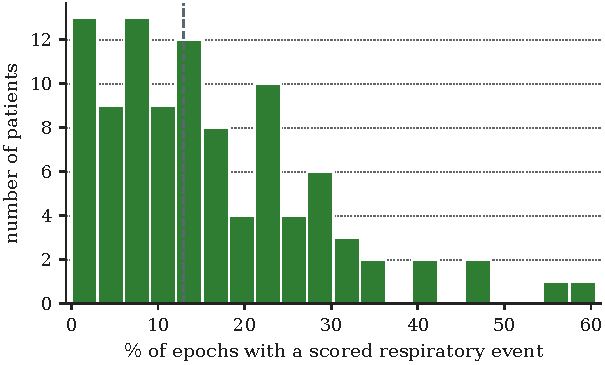
\includegraphics[width=0.86\columnwidth]{figures/fig_mm_apnea_prev.pdf}
\caption{Patient-level respiratory-event burden in iSLEEPS, measured as the
fraction of 30-s epochs containing the onset of a scored respiratory event. The dashed line
denotes the cohort median of $13\%$.}
\label{fig:prev}
\end{figure}

\subsection{Sleep-EDF: Healthy-Sleep Reference Cohort}

Sleep-EDF is used to provide a healthy-sleep reference
~\cite{kemp2000sleepedf,goldberger2000physionet}. The experiments use the
Sleep Cassette subset corresponding to subjects 0--20, comprising 40 overnight
recordings. Because individual subjects can contribute more than one night,
splits are constructed at the subject level rather than at the recording level.

Sleep-EDF serves three purposes in this study. First, it provides an independent
check of the reimplemented sleep-staging architectures against the healthy-sleep
setting in which those models were originally evaluated. Second, models trained
on Sleep-EDF are applied to iSLEEPS without adaptation to examine transfer from
healthy sleep to the stroke cohort. Third, the proposed staging model is
evaluated on Sleep-EDF as an independent healthy-sleep cohort. The database
provides frontal EEG derivations including Fpz-Cz and Pz-Oz. It does not provide
the full cardiorespiratory signal set required by the proposed respiratory
branch and contains no respiratory-event annotations used by this study;
consequently, respiratory performance is not evaluated on Sleep-EDF.

\subsection{ISRUC-Sleep: Independent Sleep-Disorder Cohort}

ISRUC-Sleep provides the independent evaluation in a population with sleep
disorders~\cite{khalighi2016isruc}. The subset used here contains eight
subjects recorded on two nights each. The recordings include central and
occipital EEG derivations corresponding to C4, C3, O2, and O1 referenced to the
contralateral mastoid, together with respiratory signals including airflow,
respiratory effort, SpO$_2$, and ECG. The dataset also contains annotations for
obstructive, central, and mixed apneas and hypopneas.

ISRUC-Sleep therefore supports evaluation of both components of the proposed
framework: sleep-stage prediction and respiratory-event prediction. The two
recording nights are retained separately in the external analysis because their
respiratory-event prevalence differs substantially. Channels required by the
iSLEEPS-trained model but unavailable in ISRUC-Sleep are represented using the
same zero-filled missing-channel convention described below.

\subsection{Signal Selection and Harmonization}

The iSLEEPS recordings contain 22 physiological and auxiliary traces. Fourteen
signals are retained for modeling and divided into neural and
cardiorespiratory groups. The neural group contains four EEG derivations
(C4:M1, C3:M2, O2:M1, and O1:M2), two EOG derivations (E1:M2 and E2:M2), and
the submental EMG. The cardiorespiratory group contains ECG, airflow, thoracic
effort, abdominal effort, summed respiratory effort, SpO$_2$, and pulse.

Signals associated with periodic limb movement, snoring, plethysmography, body
position, ambient light, and device operation are not included in the model.
The snore channel is additionally excluded from respiratory prediction because
it is closely related to the airway information used during respiratory-event
assessment. Twelve iSLEEPS recordings lack at least one selected
cardiorespiratory channel. These patients are retained, and unavailable inputs
are zero-filled rather than removing the corresponding recording. The same
convention is used when a selected signal is unavailable in an external
dataset.

The three datasets differ in montage and in the availability of
cardiorespiratory channels. Dataset-specific signal availability is therefore
preserved rather than treating the external recordings as if they contained the
complete iSLEEPS montage. Sleep-EDF is used only for analyses supported by its
available sleep-staging signals, whereas ISRUC-Sleep provides sufficient
respiratory information to evaluate the respiratory output with unavailable
inputs explicitly represented as missing channels.

\subsection{Preprocessing and Epoch Labels}

All sleep-stage predictions are defined on 30-s epochs. For iSLEEPS and
ISRUC-Sleep, the respiratory annotations are mapped to the same epoch grid. An
epoch is assigned a positive respiratory label if a scored respiratory event begins
within it and a negative label otherwise. The primary
respiratory task is therefore prediction of respiratory-event presence within
a 30-s epoch; event-level behavior is evaluated separately in
Section~\ref{sec:results}.

For the iSLEEPS neural representation, the selected EEG, EOG, and EMG signals
are resampled to $100$\,Hz for computation of the engineered descriptors
described in Section~\ref{sec:features}. The frozen LaBraM encoder is applied
only to the four EEG derivations. Because LaBraM was pretrained at $200$\,Hz,
these EEG signals are independently resampled to $200$\,Hz before entering the
pretrained encoder. The EOG and EMG channels are not supplied to LaBraM.

The seven cardiorespiratory inputs are resampled to a common $25$\,Hz grid
using polyphase resampling before entering the learned cardiorespiratory
encoder. SpO$_2$ is recorded natively at $4$\,Hz and is placed on the same
$25$\,Hz grid for temporal alignment with the remaining channels; this
operation does not increase the underlying temporal resolution of the
oximeter signal. Raw cardiorespiratory signals remain in their recorded
physical units after resampling.

Engineered feature representations are standardized within each recording
before model input. For iSLEEPS, where each analyzed patient contributes one
overnight recording, this corresponds to the patient-wise standardization used
throughout the primary analysis. The same per-recording procedure is applied
when the trained model is evaluated on the external datasets. No labels from an
external dataset are used to refit model parameters, select thresholds, or
adapt the reported iSLEEPS model.

%=====================================================================
\section{Proposed Method}
\label{sec:method}
\subsection{Problem Formulation}
A night is a sequence of $T$ epochs. For epoch $t$ we form a neural feature vector
$\mathbf{f}^{\mathrm{eeg}}_t\in\mathbb{R}^{388}$, formed by concatenating the $188$
engineered descriptors below with a $200$-dimensional embedding from LaBraM, a frozen
pretrained EEG encoder~\cite{labram2024} (Section~\ref{sec:repr}), and a raw cardiorespiratory tensor
$\mathbf{x}^{\mathrm{car}}_t\in\mathbb{R}^{7\times750}$, the seven channels at $25$\,Hz.
The $14$ engineered cardiorespiratory descriptors defined below are used by the baseline
configuration against which the learned encoder is measured.

The pretrained encoder is fed on its own terms. LaBraM was
pretrained at $200$\,Hz and fixes its input length at $3000$ samples, so the EEG is
resampled from our $100$\,Hz working rate to $200$\,Hz before it reaches the encoder.
Feeding the $100$\,Hz signal directly would have been silent but wrong: $3000$ samples
then span $30$\,seconds of recording while the encoder reads them as $15$, compressing
time by a factor of two, so every rhythm would present at twice its frequency and a
$12$\,Hz spindle would arrive as $24$\,Hz. At $200$\,Hz a $30$\,s
epoch no longer fits the positional embedding in one piece, so each epoch is split into
two $15$\,s sub-windows of $3000$ samples, encoded separately, and mean-pooled; the two
embeddings were checked to differ before caching, so the pooling carries information
and does not merely average duplicates. The encoder also requires canonical $10$--$20$ names
and rejects mastoid references, so C4:M1, C3:M2, O2:M1 and O1:M2 are presented as C4,
C3, O2 and O1, and the ocular and chin channels are dropped for having no canonical EEG
name. Amplitudes are scaled to $\mu$V$/100$. The encoder therefore sees four EEG
channels, strictly fewer signals than the engineered descriptors read. We learn a subject-independent
map
\begin{equation}
f_\theta:\big(\mathbf{f}^{\mathrm{eeg}}_{1:T},\mathbf{x}^{\mathrm{car}}_{1:T}\big)\ \longmapsto\
\big(\hat y^{\mathrm{stg}}_{1:T},\ \hat y^{\mathrm{apn}}_{1:T}\big),
\end{equation}
where $\Delta^4=\{p\in\mathbb{R}^5:p_k\geq 0,\ \sum_k p_k=1\}$ is the four-simplex,
$\hat y^{\mathrm{stg}}_t\in\Delta^4$ is a distribution over the five stages and
$\hat y^{\mathrm{apn}}_t\in[0,1]$ scores whether epoch $t$ contains a respiratory
event (Fig.~\ref{fig:arch}). We write $\hat y^{\mathrm{apn}}_t$ as a score and not as a
probability for the reason given in Section~\ref{sec:training}: the positive weighting in its
loss displaces the optimum away from the conditional event rate.

\begin{figure*}[t]
\centering
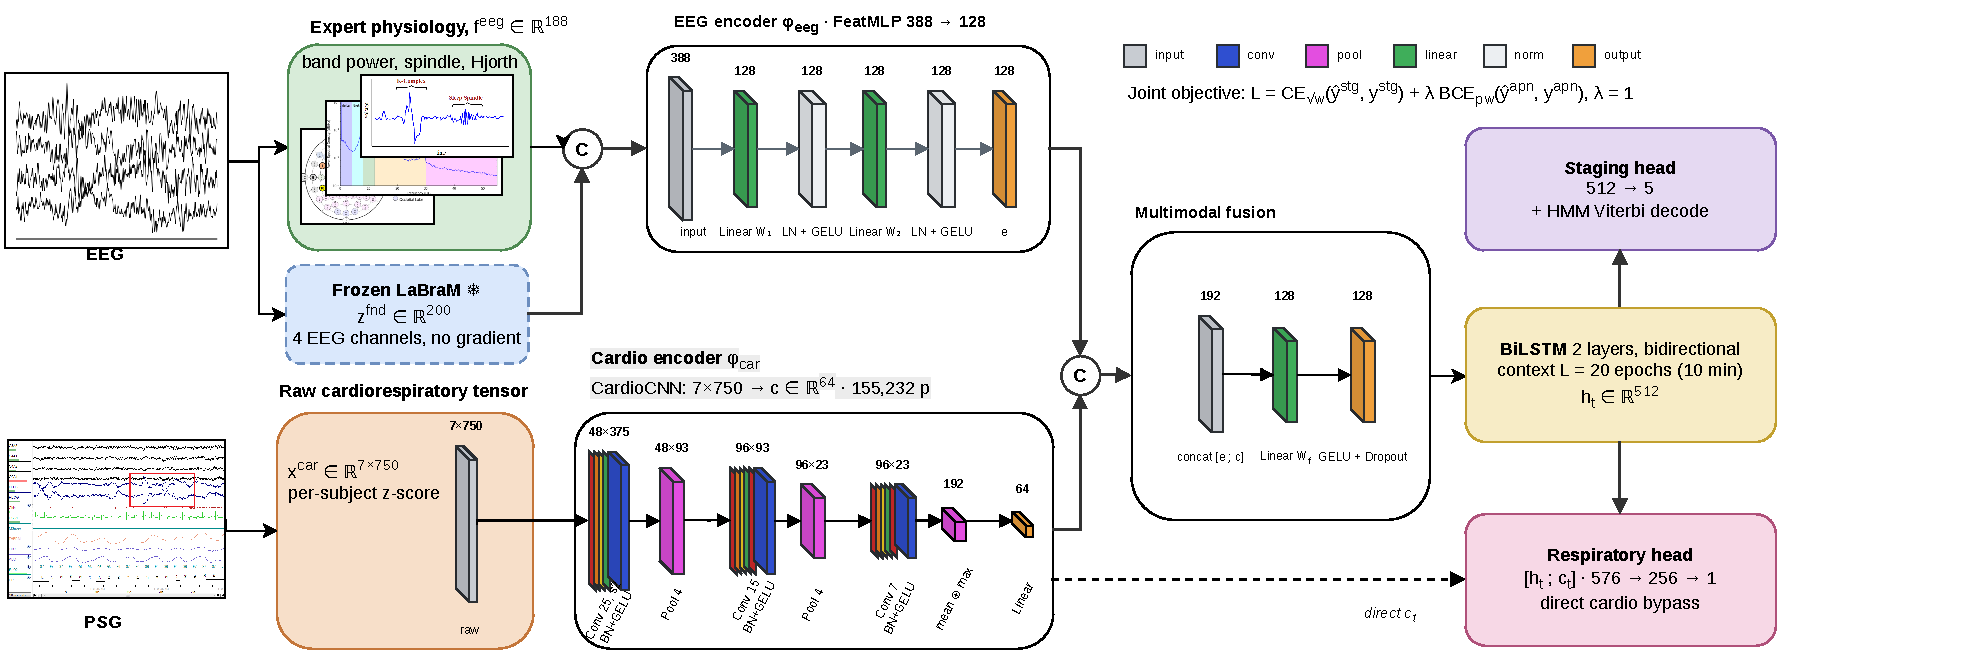
\includegraphics[width=1.1\textwidth, height=7cm]{figures/fig_architecture.pdf}
\caption{The two-stream, multi-task model. Layer shapes above each block, operation
below; block height encodes units for the multilayer perceptron and temporal length for
the convolutional stack. Dashed outlines mark frozen parameters. The junction marked C is the
concatenation used for every reported result, and the fusion panel is the single linear
layer that follows it.}
\label{fig:arch}
\end{figure*}

\subsection{Physiological Feature Representations}
\label{sec:features}
\paragraph{Neural features ($188$)}
Per channel we take absolute and relative band powers from the Welch spectrum $P(f)$ in delta
($0.5$--$4$), theta ($4$--$8$), alpha ($8$--$13$), sigma ($11$--$16$), and beta
($16$--$30$)\,Hz; the relative power in band $b$ is
\begin{equation}
\mathrm{RP}_b=\frac{\int_{f\in b}P(f)\,df}{\int_{0.5}^{30}P(f)\,df}.
\end{equation}
The bands are the conventional sleep bands and alpha and sigma overlap between $11$ and
$13$\,Hz, so the five relative powers are not a partition and do not sum to one. We keep the
conventional definitions because both bands name physiology a scorer reads, and the model
treats the five as correlated descriptors whose sum is unconstrained.
We add spectral entropy $H=-\sum_i p_i\log p_i$ with $p_i$ the normalized spectrum, the
$95\%$ spectral-edge frequency, the three Hjorth descriptors~\cite{hjorth1970eeg}, and
time-domain statistics. Sleep spindles are detected on the sigma-band analytic envelope,
the modulus of the analytic signal built from the Hilbert transform $\mathcal{H}$,
$e(t)=\lvert x_\sigma(t)+i\,\mathcal{H}\{x_\sigma\}(t)\rvert=\sqrt{x_\sigma(t)^2+\mathcal{H}\{x_\sigma\}(t)^2}$, with
density counted above a per-epoch threshold. No duration, separation or morphology criterion
is applied, so this counts crossings of a sigma-band envelope and is a proxy for spindle
density and not a validated spindle detector; the same holds for the slow-wave descriptors,
which summarise amplitude and detect nothing. Ocular-movement energy on
the EOG and tonic EMG level complete the set.

\paragraph{Cardiorespiratory features ($14$)}
From the seven cardiorespiratory channels we compute SpO$_2$ mean, minimum, variability, and
desaturation depth (median minus minimum); pulse mean and variability; ECG amplitude and
line-length; airflow amplitude and line-length; thoracic, abdominal, and summed effort
amplitudes; and signed thoraco-abdominal synchrony, whose loss is the paradoxical motion of
chest against abdomen that marks an obstructed breath. The correlation is kept signed, so
synchronous and paradoxical motion sit at opposite ends of the range; a value near $+1$ is synchronous motion and a negative value is paradox,
\begin{equation}
\mathrm{sync}_t=\mathrm{corr}(x^{\mathrm{tho}}_t,\ x^{\mathrm{abd}}_t).
\end{equation}
Both feature sets are standardized per patient, which removes person-to-person offsets so the
model generalizes across people.

\paragraph{The learned cardiorespiratory encoder}
The evaluated model does not read the $14$ descriptors. Its cardiorespiratory branch is a
three-layer convolutional encoder over the raw $7\times750$ tensor, with wide kernels and
aggressive downsampling because respiratory events are slow: at $25$\,Hz the first kernel of
$25$ samples spans one second, and a hypopnea unfolds over $10$ to $30$. Channel widths are
$48$, $96$ and $96$, each followed by batch normalisation and GELU, with max-pooling by four
after the first two. Mean and max pooling over time are concatenated and projected by a
linear layer, LayerNorm, GELU and dropout to the same
$64$ dimensions as the cardiorespiratory feature MLP it replaces, so the encoder is a drop-in replacement and every
other part of the network is unchanged. The branch holds $155{,}232$ trainable parameters,
of which the projection LayerNorm supplies $128$. Section~\ref{sec:repr} quantifies the
effect of this substitution, which is among the
largest representation changes we measure, and
Section~\ref{sec:nested} shows that the effect belongs to the change of
representation: random encoders of comparable capacity
over the same raw signal recover much of it. This encoder is used because it is small,
trained end-to-end with the rest of the network, and adds no external dependency. We
therefore attribute the observed improvement to the representation rather than to the
specific encoder architecture.

\subsection{Two-Stream Encoders}
The neural stream is a two-layer perceptron with LayerNorm; the
cardiorespiratory stream is the convolutional encoder described above, which emits a vector
of the same width the perceptron it replaced produced,
\begin{align}
e_t&=\mathrm{GELU}\!\big(\mathrm{LN}(W_2\,\mathrm{GELU}(\mathrm{LN}(W_1\mathbf{f}^{\mathrm{eeg}}_t))) \big)\in\mathbb{R}^{128},\\
c_t&=\mathrm{CardioCNN}\big(\mathbf{x}^{\mathrm{car}}_t\big)\in\mathbb{R}^{64}.
\end{align}
LayerNorm is used in place of BatchNorm because the recurrent windows are short and mix
patients within a batch, and the cardiorespiratory stream is deliberately narrower because
the branch compresses a $7\times750$ tensor into the same $64$ dimensions the
feature encoder it replaced produced, which keeps the substitution the only variable.

\subsection{Fusion}
The two embeddings are concatenated and projected back to the stream width,
\begin{equation}
z_t=\mathrm{GELU}\!\big(W_f\,[\,e_t\ ;\ c_t\,]\big)\in\mathbb{R}^{D},\qquad D=128.
\end{equation}
This is the simplest fusion available, and it is what every number in this paper
was produced with. We additionally evaluated an attention-based fusion, in which the two
embeddings are treated as tokens carrying learned modality-type embeddings, refined by
four-head scaled
dot-product attention so each modality can read the other, then projected. On the same ten
folds, in the feature-only configuration the comparison was run in, attention was
indistinguishable from concatenation on staging ($+0.005$ accuracy, $p=0.49$) and slightly
worse on the respiratory head ($-0.014$ AUC, $p=0.06$). Since the attention-based fusion
provides no measurable improvement in this setting, we report and release the simpler one,
and the gain from the second stream is therefore attributable to the added modality.

\subsection{Temporal Decoder and Two Heads}
Sleep is sequential and respiratory events cluster, so the fused vectors of an $L=20$ epoch
window ($10$ minutes) are read by a two-layer bidirectional LSTM. Training draws windows at a
stride of $L/2$, so an interior epoch is seen twice per pass and an epoch in the first or last
ten of a recording once; we apply no correction for that, and the first and last window of
each night are zero-padded to $L$ under a mask that removes the padding from the loss.
Inference uses disjoint windows: a recording is padded to a multiple of $L$, split into
consecutive blocks, and the padding discarded, so every epoch is scored exactly once and no
stitching rule is needed. Hidden states are not carried between windows in either case.
Each direction runs the
standard recurrence
\begin{align}
i_t&=\sigma(W_i[z_t,h_{t-1}]), & f_t&=\sigma(W_f[z_t,h_{t-1}]),\nonumber\\
o_t&=\sigma(W_o[z_t,h_{t-1}]), & g_t&=\tanh(W_g[z_t,h_{t-1}]),\\
s_t&=f_t\odot s_{t-1}+i_t\odot g_t, & h_t&=o_t\odot\tanh(s_t),\nonumber
\end{align}
and the forward and backward states of the $256$-unit layers are concatenated into
$h_t\in\mathbb{R}^{512}$. The
staging head is a linear map $\hat y^{\mathrm{stg}}_t=\mathrm{softmax}(W_s h_t)$. The
respiratory head reads $h_t$ together with a direct copy of the per-epoch cardiorespiratory
embedding $c_t$,
\begin{equation}
\hat y^{\mathrm{apn}}_t=\sigma\!\big(W_2\,\mathrm{GELU}(W_1[h_t;c_t])\big).
\end{equation}
The connection exists so that the respiratory decision does not have to survive a
fusion trained mostly for staging, which would weaken the mechanical signature of an
obstructed breath along the way. Section~\ref{sec:ablate} identifies the channel that
signature lives in, and it is respiratory effort that names the event. We isolate the connection by removing it and holding everything else fixed, on the
same folds as every other figure here. Respiratory AUC falls from $\mmAuc$ to
$0.776$ (Wilcoxon on ten fold-means, $p=0.049$) and average precision from $\mmAp$ to
$0.411$ ($p=0.28$), while staging is untouched at $0.739$ accuracy ($p=0.92$) and $\kappa$
$0.634$ ($p=0.92$). The gain
is small, about a sixth of a fold standard deviation, and the $p$-value is marginal, so it
does not support an argument on its own. Its relevance lies in where the effect appears: the
connection feeds the respiratory head and nothing
else, and the respiratory head is the only output that changes.

Capacity is not what produces that gain. The head reads
$2\,\text{hidden}+d_{\mathrm{card}}$ inputs whether or not the bypass is used, since the
ablation zeroes the cardiorespiratory block instead of deleting it, so both arms hold the
same $2{,}764{,}774$ parameters. A third configuration provides a stricter control by
feeding the head the same embeddings permuted across the epochs of the window, which keeps
capacity, statistics and gradient path and destroys only the alignment to the epoch. It
reaches $0.774$ AUC, at or just below the zeroed arm's $0.776$, indicating that a misaligned
cardiorespiratory signal confers no advantage over its absence. On this evidence the bypass
is a supporting design choice.

The trained model holds $2.76$ million parameters. The pretrained encoder that supplies the
$200$-dimensional neural embedding is run once offline and is not trained here, so it adds no
trainable parameters to this count.

\subsection{Training and Decoding}
\label{sec:training}
The two tasks are trained together with equal weight, $\mathcal{L}=\mathcal{L}^{\mathrm{stg}}+\lambda\,\mathcal{L}^{\mathrm{apn}}$ with $\lambda=1$, combining a class-weighted staging cross-entropy and a positive-weighted respiratory cross-entropy,
\begin{align}
\mathcal{L}^{\mathrm{stg}}&=-\sum_t\sum_{k}w_k\,y^{\mathrm{stg}}_{t,k}\log\hat y^{\mathrm{stg}}_{t,k},\\
\mathcal{L}^{\mathrm{apn}}&=-\sum_t\big[\pi\,a_t\log\hat y^{\mathrm{apn}}_t+(1-a_t)\log(1-\hat y^{\mathrm{apn}}_t)\big].
\end{align}
The staging weights use the square root of inverse class frequency,
$w_k\propto\sqrt{N/(K n_k)}$ for $K=5$ classes with $n_k$ examples, which corrects the scarce
N1 and N3 stages without giving up overall accuracy, and the respiratory term is
positive-weighted by $\pi=n_-/n_+$ to match the $16\%$ event rate, which on this corpus is
$\pi\approx5.3$.

Both weightings move the optimum, and we state where. Minimising the weighted binary term
against a true conditional rate $p$ is minimised not at $p$ but at
$q^{\star}=\pi p/[\pi p+(1-p)]$, so an epoch carrying a true event probability of $0.157$ is
driven towards $0.5$; the staging weights displace the softmax by the same mechanism, to
$q^{\star}_k\propto w_k p_k$. Neither head therefore emits a calibrated posterior, and a
threshold of $0.5$ on the respiratory output is not a fifty-per-cent event probability. Both
displacements are monotone, so ranking is untouched and the AUC and average precision we
report are unaffected; what they do affect is any reading of the numbers as probabilities,
which is why Section~\ref{sec:results} treats the outputs as scores and measures calibration
separately.

At inference the staging
posteriors are smoothed by a Viterbi pass whose transition matrix $A^{\mathrm H}$
and prior are counted from the training labels~\cite{chen2024hmm},
\begin{equation}
\delta_t(j)=\max_i\big[\delta_{t-1}(i)+\log A^{\mathrm H}_{ij}\big]+\log\hat y^{\mathrm{stg}}_t(j),
\end{equation}
recovered by back-tracking, which restores the natural persistence of sleep.

This is a transition-regularised discriminative decoder and not a generative hidden Markov
model. A generative emission term is
$\log P(\mathbf{x}_t\mid s_t=j)$, whereas $\hat y^{\mathrm{stg}}_t(j)$ is a class-weighted
discriminative score computed from a bidirectional window; inserting it in the emission slot
applies the stage prior a second time, once through $A^{\mathrm H}$ and once through the
score itself. Dividing by the prior would not repair this, because the class weights and the
recurrent context have already displaced the score from any posterior it might have been.
The pass supplies a transition prior on the output sequence, which is the property we claim
for it. The respiratory
head is left unsmoothed. Optimization uses AdamW with cosine annealing and early stopping on a
held-out set of patients.

%=====================================================================
\section{Experiments}
\label{sec:results}
\subsection{Protocol and Metrics}
All results use ten-fold, patient-independent cross-validation, so no patient appears in both
training and test, and within each training split a disjoint set of patients is held out for
early stopping. Staging is scored by accuracy, macro-F1 $\tfrac{1}{K}\sum_k\mathrm{F1}_k$, and
Cohen's $\kappa$. The respiratory task is scored by the area under the ROC curve (AUC) and
average precision (AP), which suits the $16\%$ event rate.

Every number we report is a mean over the ten folds with its standard deviation. That
standard deviation is a spread and not a confidence interval, and the distinction matters
here because the folds share training patients and are therefore dependent. The unit that
is close to independent is the patient, so we also resample patients with replacement,
$10{,}000$ times, rebuilding the pooled epoch set and recomputing every metric. That gives
$0.734$ accuracy with a $95\%$ interval of $[0.717,\ 0.750]$, $\kappa$ $0.628$
$[0.604,\ 0.651]$, respiratory AUC $0.778$ $[0.752,\ 0.802]$ and average precision $0.419$
$[0.355,\ 0.480]$. These condition on the fitted procedure: they carry the variation in
which patients were recorded and not retraining variability, and they say nothing about the
selection optimism measured below. The
folds are fixed across all configurations so that comparisons are paired. Fixing them has a
cost that we quantify below: the reported configuration was chosen by comparing forty-nine
candidates on these same ten folds, which is the standard route by which an in-domain figure
acquires selection optimism. We therefore measured how much it acquired, by repeating the
selection with the test patients held out from model selection (Section~\ref{sec:nested}): five outer
patient-independent folds, all forty-nine candidates compared on three inner folds within
each outer training set, and the winner scored once on outer patients that took no part in
choosing it. That procedure
reaches $0.734 \pm 0.009$ accuracy against the $\mmAcc$ reported here, so the optimism is
$0.006$, about a third of the fold-to-fold standard deviation of
$0.019$ and small enough that it changes no comparison in this paper. The external corpora in
Section~\ref{sec:external} took no part in selection
either, so the zero-shot figures there were never exposed to it. The proposed
model, its ablations and the retrained baselines all use the full ten; only the Sleep-EDF
transfer row was run at five, as stated in the discussion of Table~\ref{tab:bench}. Because performance estimates may vary
across random seeds, we retrained the headline configuration under three
seeds on the same folds. Staging accuracy varies by $0.005$ across seeds against
$0.020$ across folds, and respiratory AUC by $0.001$ against $0.038$: fold-to-fold spread
is four times the seed spread for staging and about thirty-four times it for respiratory detection.
The uncertainty in these results is therefore dominated by which patients fall in which
fold, which is a property of a cohort this size. Every headline figure in this paper is the mean over all thirty fold-values, ten
folds by three seeds. Paired tests, however, are computed on the ten fold-means: the three
seeds within a fold train and test on the same patients, so they constitute repeated training
runs on one patient partition, and treating them as thirty would triple
the effective sample and shrink every $p$. One consequence follows directly. With
ten paired folds the smallest two-sided Wilcoxon $p$ is $2/2^{10}=0.002$, reached when every
fold moves the same way, so after Holm correction across a family of nine the floor is
$0.018$. Several effects below sit at that floor and differ in size by more than an order of
magnitude; the test cannot separate them, and the effect sizes are reported beside every
$p$ for that reason. The comparisons of the respiratory bypass, the joint objective, the fusion
type and the incomplete-montage subgroups are secondary analyses and are reported without
multiplicity correction. The three seed means for respiratory AUC are
$0.781$, $0.783$ and $0.781$, so $\mmAuc$ is stable to the third decimal under reseeding.

\subsection{Selection Inside the Training Data}
\label{sec:nested}
The figures above are produced by a configuration chosen on the folds that score it. To find
out what that contributes we ran the whole selection again with the test patients held out
from model selection:
five outer patient-independent folds; inside each outer training set, three inner folds; all
forty-nine candidates of the original search compared on those inner folds alone; and the
inner winner retrained on the full outer training set and scored once on the outer patients.
No outer patient influences the choice of the model that scores them, so the resulting number
estimates the whole procedure, search included.

The nested procedure yields a comparable estimate, reaching
$0.7336 \pm 0.0089$ accuracy across the five outer folds against $\mmAcc$ for the reported
model. The estimated selection optimism is therefore $0.006$ accuracy, about a third of the
fold-to-fold standard
deviation and smaller than the performance differences underlying the principal comparisons.
It is also close
to the $0.004$ suggested by the spread of the top ten candidates, so the bound available
without a nested loop was of the right order.

The design the inner loop arrived at is informative in its own right. Every outer fold kept
the neural side of the published model unchanged, the engineered descriptors with the frozen
encoder, the BiLSTM, and the same width and regularisation, providing consistent support for
the neural half of the architecture across all five outer folds. Where the folds differed from the published
model was the cardiorespiratory encoder: four chose a randomly initialised time-series
encoder over the raw signal and the fifth a random projection of the fourteen engineered
descriptors, and none chose the learned convolutional encoder.

That is consistent with what Section~\ref{sec:repr} already reports from the other direction,
where a random expansion of the same fourteen numbers recovers a large part of the gap to the
learned encoder. Read together, the two experiments locate the effect: what matters is that
the cardiorespiratory stream is given a high-capacity representation of the raw signal rather
than fourteen summary statistics, and several encoders supply that equally well at this
cohort size. These results therefore attribute the observed effect to the change in
representation rather than to the specific encoder architecture. The encoder implementing it
is interchangeable at this cohort size, and the
accuracy is unaffected either way,
since every configuration the search selected lands within $0.006$ of the reported one.

Each outer model is trained jointly, so the nested procedure also yields a selection-free
estimate for the respiratory output. The five outer winners reach a respiratory AUC of
$0.774 \pm 0.047$ and an average precision of $0.406 \pm 0.077$, against $\mmAuc$ and
$\mmAp$ for the reported model, which places the selection optimism of the respiratory
output at $0.008$ AUC and $0.013$ average precision. These values are of the same order as
the staging optimism and well within the fold-to-fold standard deviation of $0.038$.
The inner loop selected on staging accuracy alone, and the lowest outer value, $0.698$, comes
from the fold in which the random projection of the fourteen descriptors was selected; the
four folds that selected the randomly initialised time-series encoder average $0.793$. The
nested estimate therefore remains well above the $0.698$ obtained with the fourteen
engineered descriptors in the same configuration (Table~\ref{tab:repr}).

Two limitations qualify this estimate. Five outer folds are fewer than the ten used
everywhere else, so it is
noisier than the figures it is compared against; and it uses a single seed, because five
outer folds by forty-nine candidates by three inner folds is already seven hundred and
thirty-five trainings.

\subsection{Implementation and Hyperparameters}
The model is implemented in PyTorch and trained on a single NVIDIA RTX~2060 GPU (6\,GB) under
Windows. Every run is seeded, so each is individually reproducible; headline figures
average three seeds ($42$, $1$, $7$) over the ten folds, giving the thirty fold-values used
throughout. Where a result is derived from stored predictions without retraining, it comes
from the seed-$42$ run, and the text says so at that point.
Table~\ref{tab:hyper} lists the training configuration, which is identical across all folds
and every ablation, so that reported differences come from the model. The six reimplemented
baselines are trained at the optimiser, batch size and schedule of their own papers, since
imposing our settings on them would understate architectures tuned for other choices.

\begin{table}[t]
\caption{Training configuration of the proposed model, shared across all folds and every
ablation. Each reimplemented baseline is trained at its own published settings instead.}
\label{tab:hyper}
\centering
\small
\begin{tabular}{ll}
\toprule
Setting & Value \\
\midrule
Framework / hardware & PyTorch, NVIDIA RTX~2060 (6\,GB) \\
Optimizer & AdamW \\
Learning rate & $3\times10^{-4}$ \\
Weight decay & $1\times10^{-4}$ \\
LR schedule & cosine annealing \\
Sequence length $L$ & $20$ epochs ($10$\,min) \\
Batch size & $32$ \\
Max epochs / patience & $45$ / $8$ \\
Gradient clipping & $5.0$ \\
Staging class weights & $\sqrt{}$ inverse-frequency \\
Respiratory pos.\ weight & $\pi=n_-/n_+$ \\
Loss balance $\lambda$ & $1.0$ \\
Staging post-processing & HMM Viterbi smoothing \\
Cross-validation & $10$-fold, patient-independent \\
Random seeds & $42$, $1$, $7$ \\
\bottomrule
\end{tabular}
\end{table}

\subsection{Compared Methods}
We compare the model against deep networks evaluated on the same folds: convolutional and
recurrent networks trained from scratch (DeepSleepNet, AttnSleep, a four-channel CNN--BiLSTM),
six further published architectures we reimplemented for this comparison (U-Time, a
fully convolutional encoder--decoder; TinySleepNet, a compact convolutional--recurrent model;
SleepTransformer, a purely attentional one; and 1D-ResNet-SE-LSTM, Micro SleepNet and
AT-BiLSTM), the released SE-ResNet-18 model of~\cite{bose2026gap}, a
network transferred from Sleep-EDF, and a raw-signal convolutional network on all $14$ channels,
alongside the published single-channel baselines for the corpus~\cite{maiti2026isleeps}. All numbers are
patient-independent, ten-fold except for the Sleep-EDF transfer row at five, at the hidden-Markov operating point where a model provides one.

\begin{table}[t]
\caption{Reimplementation check for the models marked $^{\dagger}$ in
Table~\ref{tab:bench}: ten-fold subject-independent cross-validation on the
Sleep-EDF Cassette subjects $0$--$20$, $40$ recordings, single Fpz-Cz derivation.
Every row compares accuracy except $^{\S}$U-Time, whose paper reports macro-F1 and no
accuracy for Sleep-EDF; that row therefore compares macro-F1 to macro-F1, and our U-Time
reaches $0.791 \pm 0.062$ accuracy, a quantity its paper does not state. Each published figure
follows its own paper's Sleep-EDF protocol, which differs in subset and split.}
\label{tab:reimpl}
\centering
\begin{tabular}{@{}l c c c@{}}
\toprule
Model & Published & Ours & $\Delta$ \\
\midrule
U-Time~\cite{perslev2019utime}$^{\S}$ & 0.79 & $0.660 \pm 0.054$ & $-0.130$ \\
TinySleepNet~\cite{supratak2020tinysleepnet} & 0.854 & $0.824 \pm 0.045$ & $-0.030$ \\
SleepTransformer~\cite{sleeptransformer2022} & 0.814 & $0.823 \pm 0.033$ & $+0.009$ \\
1D-ResNet-SE-LSTM~\cite{li2023resnetselstm} & 0.864 & $0.832 \pm 0.036$ & $-0.032$ \\
Micro SleepNet~\cite{liu2023microsleepnet} & 0.828 & $0.800 \pm 0.041$ & $-0.028$ \\
AT-BiLSTM~\cite{fu2021atbilstm} & 0.838 & $0.835 \pm 0.046$ & $-0.003$ \\
\bottomrule
\end{tabular}
\end{table}

\begin{table*}[t]
\caption{Sleep staging on iSLEEPS, patient-independent, against every architecture we
evaluated. Cells are mean $\pm$ SD across folds where per-fold values were retained.
$^{\dagger}$ marks a model we reimplemented and checked against its published Sleep-EDF
figure (Table~\ref{tab:reimpl}), $^{\ddagger}$ one
quoted from~\cite{bose2026gap} on its own protocol, ``feat'' engineered features.
$^{\ast}$ marks an architecture ported from its authors' released code rather than
reimplemented from a paper. The Huttunen~et~al.\ architecture has no row in
Table~\ref{tab:reimpl} because that paper reports no Sleep-EDF figure to check against, and it is the only baseline here that
scores both tasks. The SE-ResNet-18\,+\,BiLSTM row is the released model of~\cite{bose2026gap}
retrained on our folds (seed $42$, ten fold-values, decoded as released, without
hidden-Markov smoothing; Section~\ref{sec:bose}). The parameter counts of the two neural-only
rows are those of the full network with its cardiorespiratory input zeroed. Bold marks
the best value among rows run under our protocol.}
\label{tab:bench}
\centering
\begin{tabular*}{\textwidth}{@{\extracolsep{\fill}} l l c c c c c @{}}
\toprule
 & & & Healthy & \multicolumn{3}{c}{iSLEEPS (stroke)} \\
\cmidrule(lr){4-4}\cmidrule(lr){5-7}
Model & Input & Params\,$\downarrow$ & Acc & Acc\,$\uparrow$ & Macro-F1\,$\uparrow$ & $\kappa$\,$\uparrow$ \\
\midrule
\multicolumn{7}{@{}l}{\emph{Deep networks, retrained on iSLEEPS}}\\[1pt]
LSTM, our reimplementation$^{\dagger}$ & 1\,EEG\,$+$\,EOG & $1.16$\,M & --- & $0.720 \pm 0.032$ & $0.626 \pm 0.028$ & $0.599 \pm 0.043$ \\
CNN-ResNet18~\cite{bose2026gap}$^{\ddagger}$ & 1\,EEG & $\sim$11\,M & --- & 0.617 & 0.544 & 0.480 \\
SE-ResNet-18\,+\,BiLSTM~\cite{bose2026gap}$^{\ast}$ & 1\,EEG & $11.32$\,M & $0.829 \pm 0.056$ & $0.696 \pm 0.038$ & $0.606 \pm 0.032$ & $0.572 \pm 0.046$ \\
DeepSleepNet~\cite{supratak2017deepsleepnet}  & 4\,EEG  & $3.72$\,M  & $0.823 \pm 0.050$ & $0.669 \pm 0.031$ & $0.624 \pm 0.026$ & $0.558 \pm 0.035$ \\
U-Time~\cite{perslev2019utime}$^{\dagger}$ & 1\,EEG & $1.07$\,M & $0.791 \pm 0.062$ & $0.646 \pm 0.064$ & $0.524 \pm 0.057$ & $0.506 \pm 0.082$ \\
AttnSleep~\cite{eldele2021attnsleep}          & 1\,EEG  & $\sim$0.5\,M & $0.833 \pm 0.042$ & $0.716 \pm 0.042$ & $0.600 \pm 0.043$ & $0.593 \pm 0.058$ \\
TinySleepNet~\cite{supratak2020tinysleepnet}$^{\dagger}$ & 1\,EEG & $1.45$\,M & $0.824 \pm 0.045$ & $0.676 \pm 0.050$ & $0.587 \pm 0.034$ & $0.548 \pm 0.062$ \\
SleepTransformer~\cite{sleeptransformer2022}$^{\dagger}$ & 1\,EEG & $2.79$\,M & $0.823 \pm 0.033$ & $0.683 \pm 0.026$ & $0.602 \pm 0.030$ & $0.555 \pm 0.032$ \\
1D-ResNet-SE-LSTM~\cite{li2023resnetselstm}$^{\dagger}$ & 1\,EEG & $0.65$\,M & $0.832 \pm 0.036$ & $0.708 \pm 0.038$ & $0.631 \pm 0.033$ & $0.592 \pm 0.050$ \\
Micro SleepNet~\cite{liu2023microsleepnet}$^{\dagger}$ & 1\,EEG & $0.03$\,M & $0.800 \pm 0.041$ & $0.647 \pm 0.049$ & $0.558 \pm 0.028$ & $0.510 \pm 0.055$ \\
AT-BiLSTM~\cite{fu2021atbilstm}$^{\dagger}$ & 1\,EEG & $0.92$\,M & $0.835 \pm 0.046$ & $0.692 \pm 0.040$ & $0.612 \pm 0.030$ & $0.570 \pm 0.051$ \\
CNN\,+\,BiLSTM                                & 4\,EEG  & $\sim$0.6\,M & $0.806 \pm 0.041$ & $0.670 \pm 0.052$ & $0.618 \pm 0.044$ & $0.553 \pm 0.062$ \\
Sleep-EDF transfer                            & 4\,EEG  & $\sim$0.6\,M & --- & $0.623 \pm 0.020$ & 0.582 & 0.488 \\
Raw multimodal CNN                            & 14\,ch  & 0.95\,M      & --- & $0.677 \pm 0.035$ & $0.633 \pm 0.025$ & $0.563 \pm 0.041$ \\
Huttunen~et~al.~\cite{huttunen2023simultaneous}$^{\ast}$ & 4\,ch & $3.80$\,M & --- & $0.599 \pm 0.060$ & $0.495 \pm 0.067$ & $0.440 \pm 0.078$ \\
\addlinespace[2pt]\midrule
\multicolumn{7}{@{}l}{\emph{Trained on healthy sleep, applied zero-shot}}\\[1pt]
CNN                                           & 4\,EEG  & $0.49$\,M    & $0.806 \pm 0.001$ & $0.307 \pm 0.016$ & $0.223 \pm 0.013$ & $0.102 \pm 0.010$ \\
CNN\,+\,BiLSTM (CRNN)                         & 4\,EEG  & $1.15$\,M    & $0.828 \pm 0.005$ & $0.312 \pm 0.012$ & $0.253 \pm 0.006$ & $0.127 \pm 0.022$ \\
StagingSeqNet                                 & 4\,EEG  & $1.08$\,M    & $0.855 \pm 0.001$ & $0.306 \pm 0.009$ & $0.230 \pm 0.014$ & $0.091 \pm 0.015$ \\
\addlinespace[2pt]\midrule
\multicolumn{7}{@{}l}{\emph{Proposed feature-based multi-task model}}\\[1pt]
MM-Net (neural only)              & 7\,ch feat  & 2.76\,M & --- & $\mathbf{0.741 \pm 0.017}$ & $0.668 \pm 0.020$ & $\mathbf{0.635 \pm 0.022}$ \\
\textbf{MM-Net (neural + cardio)} & 7\,ch feat $+$ raw & 2.76\,M & --- & $0.739 \pm 0.020$ & $\mathbf{0.670 \pm 0.020}$ & $0.634 \pm 0.024$ \\
\addlinespace[2pt]\midrule
\multicolumn{7}{@{}l}{\emph{Same model, healthy sleep}}\\[1pt]
MM-Net (neural only)              & 2\,EEG feat & 2.76\,M & $\mathbf{0.856 \pm 0.027}$ & --- & --- & --- \\
\bottomrule
\end{tabular*}
\end{table*}

\subsection{Staging Benchmark and Comparison}
The row marked $^{\ddagger}$ is quoted from~\cite{bose2026gap} and follows that paper's
protocol over $N=100$, which includes the duplicated pair we exclude (Section~\ref{sec:data});
the same authors' released SE-ResNet-18 model is retrained on our folds in
Section~\ref{sec:bose}. Each reimplementation is checked against the figure its own paper
publishes on Sleep-EDF (Table~\ref{tab:reimpl}); those figures follow each paper's own protocol, which
differs in subset and split, so they are consistency checks.
Our own split uses one subject more than the conventional Sleep-EDF-20 set, and one of the
published figures is measured on SHHS, so those two checks are weaker
than the rest. A third is weaker still. U-Time publishes macro-F1 and not accuracy, so its
row is the only one compared in macro-F1, and there our reimplementation sits $0.130$ below
the published figure. Macro-F1 is governed by N1, the stage whose prevalence moves most
between Sleep-EDF subsets, and the published figure comes from the $39$-recording subset
under twenty-fold cross-validation against our $40$ recordings under ten. The discrepancy
cannot be attributed reliably to reimplementation error, because the evaluation protocols
differ substantially, and we therefore do not treat this row as a direct quantitative
comparison.
Table~\ref{tab:bench} is organised in three blocks: architectures retrained on this
cohort, architectures trained on healthy sleep and applied to it zero-shot, and the
proposed model, with a final row cross-validating the proposed architecture on healthy
sleep as a control on the cohort argument; its macro-F1 and $\kappa$ are healthy-sleep
figures and so are left out of the stroke columns, and quoted in the text instead.
Dispersion is reported wherever it is defined: five folds for the Sleep-EDF transfer row;
ten fold-values (seed $42$) for DeepSleepNet, the CNN\,+\,BiLSTM, the raw multimodal CNN and
the SE-ResNet-18 model; thirty fold-values, ten folds by three seeds, for AttnSleep, the
reimplemented literature models and the proposed rows. CNN-ResNet18 is quoted
from~\cite{bose2026gap} and was not re-run here, so its protocol is that paper's and it
carries no interval. That paper's LSTM appears only as our reimplementation of it on the
folds used throughout, because its published figure was never measured on these folds. In the zero-shot block the interval is across
pretraining seeds and not folds, because that evaluation is a single pass of a finished
checkpoint over all $99$ patients. The two best healthy scores, $0.856$ and $0.855$, are
separated by less than either interval. Sleep-EDF carries none of the cardiorespiratory
channels this model reads, its Cassette recordings providing an oronasal airflow trace at
$1$\,Hz but no ECG, effort belts or oximetry and no scored respiratory events, so every
healthy-sleep figure exercises the neural branch alone and the comparison row there is
MM-Net (neural only).

Table~\ref{tab:bench} shows a clear pattern: every deep network, whether trained from scratch,
transferred from healthy sleep, or applied to the raw multichannel signal, stays between $0.60$
and $0.72$ accuracy, $12$ to $20$ points below the same architectures' published accuracy on
healthy sleepers. The feature-based model reaches $\mmAcc$, above every deep architecture we
retrained here, which matches the concurrent finding that depth alone does not help on this
cohort~\cite{bose2026gap}: with under a hundred patients a convolutional network cannot
recover the physiological structure the engineered descriptors encode explicitly, which
suggests that those descriptors supply useful inductive structure at this sample size. The corpus paper's own recurrent
baseline, reimplemented here and run on the same folds, reaches $0.720 \pm 0.032$ over
thirty fold-values. Staging performance remains within a narrow range across the evaluated
methods: nothing we have run on this
corpus exceeds $0.75$. Section~\ref{sec:curve} reports evidence consistent with this
observation, in that the staging learning curve has flattened.
We therefore do not position the model as a staging leader. Its principal distinction is
the additional respiratory output. Of the models that stage competitively here it is the only one that also
detects respiratory events; the raw multimodal CNN produces both outputs but stages at
$0.677$ with a respiratory AUC of $0.735$.

The comparison that speaks to this directly is against Huttunen~et~al., the closest prior
system: one network scoring sleep stages and respiratory events at once, which makes it the
only baseline in Table~\ref{tab:bench} that answers the same two questions this model does.
We ported the architecture from the authors' released code, so the
encoder blocks, the squeeze-and-excitation ratios, the atrous pyramid at the bottleneck and
the shape of the two segment classifiers are theirs. On the same folds it reaches
$0.599$ accuracy and $0.710$ respiratory AUC against $\mmAcc$ and $\mmAuc$, and the
proposed model is ahead in all ten folds on every metric (Wilcoxon on fold-means, $p=0.002$,
the floor at this sample size).

That margin should be read as a statement about this corpus.
Their model was built for, and reported on, $877$ suspected-obstructive-sleep-apnea
recordings; three things had to change to bring it here. The port reads four of the five
signals of their fullest configuration (SpO$_2$, oronasal airflow, summed respiratory effort
and one EEG derivation), without nasal pressure; their
respiratory output is a three-way decision every second, which this corpus cannot supply and
which we replaced with the same per-epoch binary label used throughout; and a single EEG
derivation at their $32$\,Hz is a thin neural input for staging, which is most of why the
staging gap is wider than the respiratory one. The row supports the conclusion that a joint
architecture tuned on a general sleep-apnea population does not transfer to a stroke cohort
of this size, which is the same conclusion the rest of Table~\ref{tab:bench} reaches for
single-task architectures.

A representative held-out night is
shown in Figure~\ref{fig:hypno}: the predicted hypnogram follows the reference through the
night's cycles, and the stage-probability ribbon exposes where the model is confident and where
it hesitates.

The margin over the retrained baselines is tested. The folds are fixed
across every model in Table~\ref{tab:bench}, so each baseline is scored on exactly the patients
the proposed model was and the comparison is paired. That matters here: fold-to-fold variation
is large and it is \emph{shared}, because the difficulty lies in the patients (AttnSleep spans $0.627$ to $0.755$ across folds). Since that variability is common to models evaluated on
identical patient partitions, paired comparisons are more informative than the overlap
between marginal standard-deviation ranges.
Paired on the ten fold-means, with Holm correction across the eight baselines we ran
ourselves, the proposed model is ahead of every one of them on accuracy, by $+0.019$ to
$+0.093$, and wins between eight and ten of the ten folds in each comparison. The margin is
statistically separable for five: Micro SleepNet, SleepTransformer, U-Time, AT-BiLSTM and
TinySleepNet (Holm $p$ from $0.016$ to $0.039$). For the three closest it is not. AttnSleep
($+0.023$, Holm $p=0.17$), our reimplementation of the corpus LSTM ($+0.019$, $p=0.17$) and
1D-ResNet-SE-LSTM ($+0.032$, $p=0.15$) fall within the resolution of ten folds. This is
consistent with the cohort-difficulty argument made elsewhere:
three architectures spanning 2021 to 2023 land close enough to the proposed model that this
cohort does not separate them.
The accuracy margin is the narrowest of the three and the one most exposed to the cohort's
noise. Macro-F1 and $\kappa$ show separations two to three times larger, since they reduce
the influence of performance on the two majority classes.

\begin{figure*}[t]
\centering
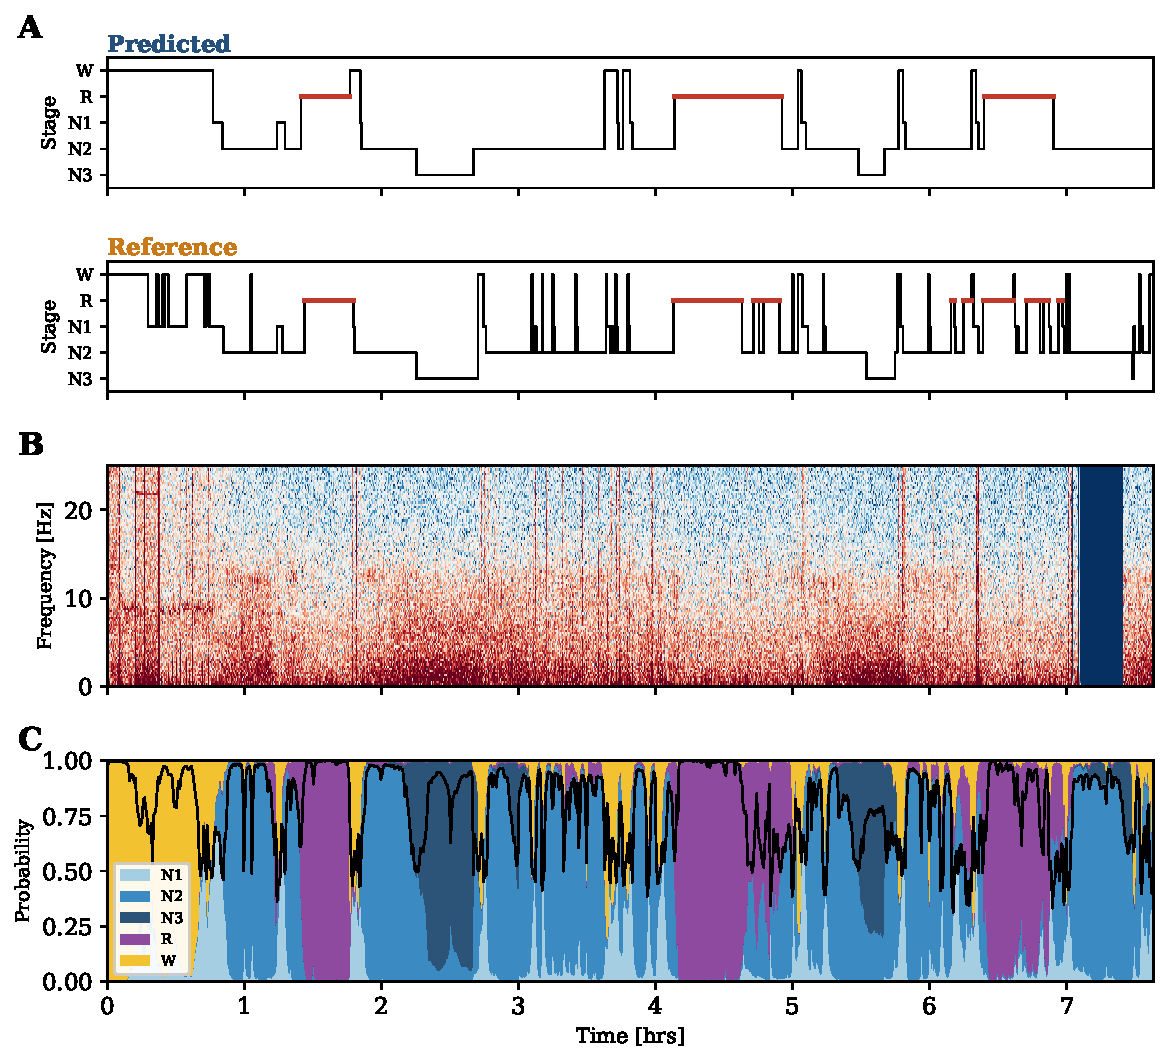
\includegraphics[width=0.86\textwidth]{figures/fig_hypnogram.pdf}
\caption{A representative held-out night (patient SN90, staging accuracy $0.81$).
\textbf{(A)} Predicted and reference hypnograms, REM highlighted. \textbf{(B)} EEG
spectrogram, C4 derivation, $0$--$25$\,Hz. \textbf{(C)} Per-epoch stage-probability
ribbon; the black line is the maximum posterior.}
\label{fig:hypno}
\end{figure*}


\subsection{The Released SE-ResNet-18 Model on the Same Folds}
\label{sec:bose}
Bose~\emph{et al.}~\cite{bose2026gap} report $74.7\%$ accuracy, $0.677$ macro-F1 and
$\kappa=0.64$ on iSLEEPS for an SE-ResNet-18 encoder followed by a bidirectional LSTM,
using the single C4:M1 derivation. Because this figure exceeds the proposed model on all
three metrics, we retrained the authors' released implementation on the folds used
throughout this paper. The architecture was taken from their released notebook without
modification: an SE-ResNet-18 epoch encoder with kernel-7 residual blocks and
squeeze-and-excitation, a $512$-dimensional epoch embedding, a six-layer bidirectional
LSTM with $100$ hidden units over windows of nine epochs, a read-out at the sixth position
of the window, and a $2000$--$200$--$5$ classification head, trained with an unweighted
negative log-likelihood, Adam at a learning rate of $10^{-3}$, a batch size of $32$ and ten
epochs, with training windows cut at a stride of four epochs. The released code builds six
LSTM layers where the paper states three; we followed the code. Four aspects of the protocol
were aligned with the rest of Table~\ref{tab:bench}: the $99$-patient folds, a checkpoint
selected on a validation split drawn from the training patients, scoring of every epoch of
every test night, and a shuffled training loader. The model has $11.32$ million parameters.

On the same ten folds it reaches $0.696 \pm 0.038$ accuracy, $0.606 \pm 0.032$ macro-F1 and
$\kappa = 0.572 \pm 0.046$ (single seed). Adding the hidden-Markov decoder used by the other
rows leaves accuracy unchanged ($0.696$) and lowers macro-F1 to $0.580$, so the row reports
the model decoded as released. Paired on the ten folds, the proposed model is higher in
accuracy by $0.044$ (nine of ten folds, Wilcoxon $p=0.010$), in macro-F1 by $0.065$ (ten of
ten, $p=0.002$) and in $\kappa$ by $0.062$ (nine of ten, $p=0.004$). The retrained model
therefore falls within the range of the other retrained baselines. On healthy sleep, run on
the same Sleep-EDF folds as the other rows, the same code reaches $0.829 \pm 0.056$ accuracy,
so the architecture performs as expected on the population it was designed for.

The published figure was obtained under a different evaluation protocol, and the two numbers
should not be compared directly. In the released notebook the checkpoint of each fold is
selected on the macro-F1 of the validation patients whose metrics are then reported, a
held-out subset of patients is used to choose among the ten fold models, evaluation windows
are cut at a stride of four epochs with incomplete batches dropped, so that not every epoch
is scored, and all $100$ recordings are used, including the duplicated pair excluded here
(Section~\ref{sec:data}).

\subsection{Per-class Staging Performance}
Table~\ref{tab:perclass} breaks staging down by stage. The pattern is the one this cohort
imposes on every method: N2, Wake, and REM are recovered well, N3 is moderate, and N1 is the
hard stage, because it is transient and rare. The raw convolutional network reaches the highest
N1 F1, which fits its sensitivity to short events, while the proposed model leads on the stable
stages. The row-normalised confusion matrix (Fig.~\ref{fig:confusion}) shows
where the errors land: N1 is absorbed mainly into Wake and N2, and part of N3 is read as N2.
Comparing the neural-only and full rows isolates what the cardiorespiratory stream
contributes to staging, and the answer is that it contributes nothing measurable. Overall
accuracy is $0.741$ without the stream and $\mmAcc$ with it; per stage, N1 improves by
$0.019$ (Wilcoxon $p=0.11$ on ten fold-means) and no stage changes significantly
($p \geq 0.15$; REM shifts by $0.01$ in Table~\ref{tab:perclass}, well inside that).

This is consistent with the physiology. Sleep stages are scored from cortical, ocular and
muscular activity, none of which the cardiorespiratory channels observe, so the absence of a
staging gain is the expected result. The clinically relevant quantity is the pair taken
together: the second stream yields respiratory-event detection at $\mmAuc$ AUC while staging
is unchanged, so the second output is obtained without a reduction in the first. The
modality-ablation grid of Section~\ref{sec:ablate} shows the same separation by the
complementary experiment, each stream supporting the output its physiology is closest to.
That the small staging gain
lands on N1 is also consistent with its physiology: it is the transitional stage, the hardest
to score, and the one most often coincident with a respiratory event.

\begin{figure}[t]
\centering
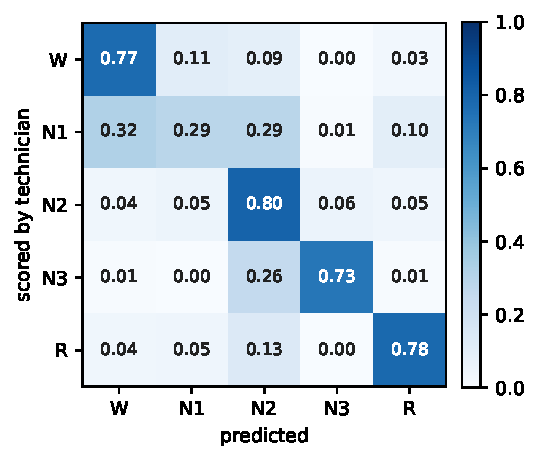
\includegraphics[width=0.82\columnwidth]{figures/fig_confusion.pdf}
\caption{Row-normalised confusion matrix for the proposed model (pooled ten-fold test epochs,
hidden-Markov operating point). Errors concentrate on N1, which is absorbed into Wake and N2.}
\label{fig:confusion}
\end{figure}

\begin{table}[t]
\caption{Per-class staging F1 (Wake, N1, N2, N3, REM), ten-fold patient-independent, at the
hidden-Markov operating point. The neural-only and full rows are means over the same thirty
fold-values. Best per column in \textbf{bold}.}
\label{tab:perclass}
\centering
\setlength{\tabcolsep}{6pt}
\begin{tabular}{lccccc}
\toprule
Model & W\,$\uparrow$ & N1\,$\uparrow$ & N2\,$\uparrow$ & N3\,$\uparrow$ & R\,$\uparrow$ \\
\midrule
Raw multimodal CNN                & 0.74 & \textbf{0.37} & 0.73 & 0.56 & 0.67 \\
MM-Net (neural only)              & \textbf{0.79} & 0.28 & 0.80 & 0.71 & \textbf{0.76} \\
\textbf{MM-Net (neural + cardio)} & 0.79 & 0.30 & \textbf{0.80} & \textbf{0.71} & 0.75 \\
\bottomrule
\end{tabular}
\end{table}

\subsection{Modality-Ablation Grid}
\label{sec:ablate}
This ablation is also our attribution method. Because the model is feature-based and never sees
a raw spectrogram or a raw EEG trace, a gradient heat-map or Grad-CAM would have no
faithful spatial support on the neural side, which is where a staging attribution would be
read; we
therefore attribute each output by \emph{interventional} ablation, deleting a physiological
channel and measuring the change. This is a falsifiable test of what each modality contributes.
The proposed model stages sleep at $\mmAcc$ accuracy ($\kappa$ $\mmK$) and detects respiratory
events at $\mmAuc$ AUC ($\mmAp$ average precision). To test the paper's central claim, that each
modality carries the task its physiology is closest to, we remove each modality in turn and keep the
rest, on the same folds, with three seeds giving thirty fold-values per row
(Table~\ref{tab:ablate}). The results show a task-specific separation between streams. Within the
cardiorespiratory stream the pattern is not the one the engineered features gave.

Removing the whole cardiorespiratory stream drops respiratory AUC from $\mmAuc$ to $0.654$,
the largest single effect in this study, and leaves staging untouched ($0.741$, n.s.).
Removing the neural stream does the reverse: staging falls from $\mmAcc$ to $0.680$ while
respiratory detection holds. No neural ablation significantly moves respiratory AUC and no
cardiorespiratory ablation significantly moves staging, so each stream serves the outcome its physiology is closest to.

Within the cardiorespiratory stream, however, only respiratory effort is individually necessary
($-0.038$ AUC, Holm $p=0.018$). Removing SpO$_2$, pulse/HRV, ECG or airflow individually costs
at most $0.005$ AUC and none survives correction; SpO$_2$, which the engineered-feature
configuration was built around, is here among the least necessary channels
($-0.002$, $p=1.00$). The five
individual removals sum to $-0.046$ AUC against $-0.128$ for removing the stream as a whole,
a factor of $2.8$. The learned encoder therefore distributes respiratory information redundantly
across channels: each is individually dispensable because the others overlap it, while the
ensemble is essential. That redundancy is clinically favourable, since
twelve of the ninety-nine recordings are missing at least one cardiorespiratory channel, and it is
physiologically coherent: the effort belts register the paradoxical thoraco-abdominal motion
of an obstructive event as it happens, whereas desaturation is a lagged consequence of it.

\subsection{What the Joint Objective Contributes}
\label{sec:joint}
The ablation grid establishes which physiology carries which output. It does not establish
whether the two outputs should share a network at all: a
model producing two outputs demonstrates integration, and integration alone does not
demonstrate benefit. The control is a
pair of single-task models, and it has to be matched properly or it measures the wrong
thing. Ours changes one line. The architecture, the ten folds, the three seeds, the
optimiser, the budget and the cardiorespiratory bypass are those of the full model; only the
surviving term of $\mathcal{L}=\mathcal{L}^{\mathrm{stg}}+\lambda\mathcal{L}^{\mathrm{apn}}$
differs, so the staging-only model still builds the cardiorespiratory stream and still feeds
the respiratory head and simply never receives a respiratory gradient. What separates the
rows is the objective.

Training both tasks together is better than training either alone
(Table~\ref{tab:joint}). Staging rises from $0.733$ to $\mmAcc$ accuracy, in nine folds of
ten (Wilcoxon on the ten fold-means, $p=0.014$), and $\kappa$ from $0.625$ to $\mmK$ on the
same nine. Respiratory AUC rises from $0.774$ to $\mmAuc$ in seven folds of ten ($p=0.049$).
Average precision moves $+0.005$ and does not separate ($p=0.63$), which we report as the
null it is.

Two readings of that are available and only the narrower one is supported. The gains are
small: $0.006$ accuracy against a fold-to-fold SD of $0.019$, and $0.007$ AUC against
$0.038$, so roughly a third and a fifth of the spread the cohort already imposes. What
carries them is consistency, nine and seven folds of ten moving the same
way, which is what the paired test is reading. The claim we make is therefore that the
second task costs the first nothing and returns a little to it, which is the claim the
architecture needs: a clinician gets the respiratory read-out without trading away staging
accuracy for it. We do not claim multi-task learning as a source of large gains here.

The two diagnostic cells are what make the comparison trustworthy. The respiratory-only
model stages at $0.303$ accuracy and $\kappa$ $0.039$, and the staging-only model detects at
$0.495$ AUC. Both are chance for their untrained head, which confirms that the switch
isolated the loss and did not quietly leave the other objective running.

\begin{table}[t]
\caption{The joint objective against matched single-task models, ten-fold
patient-independent, three seeds. Every row shares the architecture, folds, seeds and
budget; only the surviving loss term differs. $p$ is Wilcoxon on the ten fold-means, the
unit used throughout. The upper cells of each block are the metric that model was trained
for; the lower, in grey, are its untrained head and are chance by construction.}
\label{tab:joint}
\centering
\small
\setlength{\tabcolsep}{5pt}
\begin{tabular}{llccc}
\toprule
Trained on & Metric & Single & Joint & $p$ \\
\midrule
\multirow{2}{*}{Staging only}
 & Accuracy & $0.733$ & $\mathbf{\mmAcc}$ & $\mathbf{0.014}$ \\
 & $\kappa$ & $0.625$ & $\mathbf{\mmK}$   & $\mathbf{0.014}$ \\
\addlinespace[2pt]
\multirow{2}{*}{Respiratory only}
 & AUC & $0.774$ & $\mathbf{\mmAuc}$ & $\mathbf{0.049}$ \\
 & AP  & $0.414$ & $0.419$           & $0.63$ \\
\midrule
\multicolumn{5}{@{}l}{\emph{Untrained heads, reported as the check that the switch worked}}\\[1pt]
Respiratory only & Accuracy & $0.303$ & --- & --- \\
Staging only     & AUC      & $0.495$ & --- & --- \\
\bottomrule
\end{tabular}
\end{table}

\subsection{Recordings With an Incomplete Montage}
Those twelve recordings are scored with the absent channels zero-filled instead of being
excluded, which raises a fair question: does the network read missingness instead of
physiology? It does not appear to. Removing all twelve from the pooled respiratory
evaluation moves AUC from $0.777$ to $0.775$ and moves average precision the other way,
from $0.419$ to $0.439$, so the respiratory result does not rest on them. Predicted
per-patient burden is independent of whether a montage was complete ($p=0.91$), so the
shortcut is not available even in principle.

Staging is lower on those twelve, $0.670$ against $0.743$ ($p=0.017$), which calls for a
control. The neural-only configuration receives no
cardiorespiratory channel at all and so has nothing zero-filled, yet it shows the same
gap in the same direction, $0.689$ against $0.744$ ($p=0.040$). Most of the difference
therefore belongs to the recordings, which are harder for a model that cannot see the
missing channels either. On those twelve the
full model sits $0.019$ below neural-only, which at $n=12$ is not distinguishable from
noise (Wilcoxon $p=0.18$), so a small cost can be bounded but not excluded. On the
eighty-seven complete recordings the two agree to within $0.002$.

Because a zero-filled channel is indistinguishable from a flat channel after per-patient
standardisation, we also tested two explicit treatments of missing inputs, each retrained on
the same folds with seed $42$. In the first, the seven per-recording channel-availability flags
are appended to the pooled features of the cardiorespiratory encoder. In the second, the same
flags are combined with channel dropout during training, in which each available channel and
its flag are removed with probability $0.15$. The re-run of the published configuration under
the same seed reaches $0.734$ accuracy and $0.779$ respiratory AUC, with $0.779$ AUC on the
$87$ complete recordings and $0.791$ on the $12$ incomplete ones. With availability flags the
corresponding values are $0.739$, $0.782$, $0.776$ and $0.835$, and with flags and channel
dropout $0.738$, $0.779$, $0.770$ and $0.826$. Neither treatment changes the pooled results,
and both raise respiratory AUC on the incomplete recordings by about $0.04$; with twelve
patients and one seed, this difference is an indication rather than an established effect.
Attention and plain concatenation stage and detect alike, so the gain comes from the added
modality, and the fusion mechanism has little effect.

\begin{table*}[t]
\caption{Modality-ablation grid (leave-one-out), ten-fold patient-independent,
three seeds. Each row removes one modality and keeps the rest; cells are means over
thirty fold-values. $p$ is Wilcoxon on the ten fold-means, Holm-corrected across the
nine ablations within each metric and \textbf{bold} where it clears $0.05$; the
floor at this sample size is $0.018$.}
\label{tab:ablate}
\centering
\setlength{\tabcolsep}{14pt}
\begin{tabular}{lcccc}
\toprule
Modality removed & Staging acc\,$\uparrow$ & Holm $p$ & Respiratory AUC\,$\uparrow$ & Holm $p$ \\
\midrule
 none (full model)        & $0.739 \pm 0.020$   & ---                 & $0.782 \pm 0.038$   & --- \\
 EEG (neural)             & $0.680$             & $\mathbf{0.018}$    & $0.774$             & $0.92$ \\
 EOG (ocular)             & $0.731$             & $0.08$              & $0.777$             & $1.00$ \\
 EMG (muscle)             & $0.735$             & $1.00$              & $0.778$             & $1.00$ \\
 SpO$_2$                  & $0.742$             & $1.00$              & $0.780$             & $1.00$ \\
 respiratory effort       & $0.741$             & $1.00$              & $0.744$             & $\mathbf{0.018}$ \\
 pulse / HRV              & $0.741$             & $1.00$              & $0.785$             & $1.00$ \\
 ECG                      & $0.737$             & $1.00$              & $0.777$             & $1.00$ \\
 airflow                  & $0.740$             & $1.00$              & $0.778$             & $1.00$ \\
 all cardiorespiratory    & $0.741$             & $1.00$              & $0.654$             & $\mathbf{0.018}$ \\
\bottomrule
\end{tabular}
\end{table*}

\subsection{Physiological Validity of the Respiratory Read-out}
\label{sec:noflow}
Because the events were scored from airflow, predominant reliance on that channel could
produce a circular association. Removing the airflow features leaves detection essentially
unchanged, at $\noflowAuc$ AUC (Table~\ref{tab:ablate}), within one fold standard deviation of
the full $\mmAuc$, so airflow can be replaced by the other scoring-relevant channels.
Respiratory effort provides the strongest contribution, being the only channel whose removal
costs significantly, while the remaining channels are individually replaceable because the
learned encoder represents them redundantly. This indicates that detection is supported by
physiological correlates of disordered breathing rather than by reproduction of the primary
scoring signal. It is also the physiologically expected one: the effort belts register the
paradoxical thoraco-abdominal motion of an obstructive event while it is happening, whereas
desaturation follows it by several breaths.

\subsection{Respiratory Baselines and Per-event-type Detection}
The respiratory task needs real competitors (Table~\ref{tab:resp}), on the same folds.
The classical baselines read the $14$ engineered cardiorespiratory descriptors; the proposed
model reads the raw signal through its learned encoder, and its own score on the $14$
descriptors is $0.698$ (Table~\ref{tab:repr}), which is the like-for-like comparison. A clinical desaturation rule reaches $0.596$ AUC, logistic
regression $0.582$, and gradient boosting $0.670$; a random classifier scores $0.157$ average
precision, the event prevalence. The proposed model reaches $\mmAuc$ AUC and $\mmAp$ average
precision, above gradient boosting but by a modest margin, so the contribution is the joint
single pass and the physiological attribution above; we do not claim state-of-the-art
detection accuracy. Detection also separates by event type: the model scores $0.748$ AUC on hypopneas (the
mild, dominant $81\%$ of events), $0.898$ on obstructive apneas, and $0.935$ on central apneas.
It is strongest on the most severe events, and the overall AUC is held down by the abundant
hypopneas.

Two raw-signal respiratory detectors were added to test the representation argument against
networks that are trained end to end on the waveforms. Each is a per-epoch convolutional
encoder over the $25$\,Hz signal followed by a bidirectional LSTM across $20$-epoch windows,
trained on the same per-epoch label, folds and early-stopping rule as the proposed model,
with the positive class weighted by $n_-/n_+$. The first reads the summed respiratory-effort
channel alone, the input configuration of Nassi~\emph{et al.}~\cite{nassi2022effortbelt};
the second reads all seven raw cardiorespiratory channels. With a single seed, the
effort-only detector reaches $0.605 \pm 0.042$ AUC and $0.240$ average precision, and the
seven-channel detector $0.735 \pm 0.038$ AUC and $0.361$ average precision
(Table~\ref{tab:resp}). Both remain below the proposed model, which reads the same seven
channels and additionally has access to the neural stream and the shared temporal context.

\begin{table}[t]
\caption{Event-level detection, pooled over the ten patient-independent folds
($8{,}400$ scored events over $771$ hours). Within a patient an event is a maximal run of
consecutive epochs, with no gap tolerance, and counts as detected when any epoch inside it
is flagged; a false alarm is a flagged run overlapping no scored epoch, and the rate
denominator is the whole recording, wake included. One flagged run spanning several events
therefore marks each detected while costing at most one false alarm, which is where the
under-counting below comes from. The flagged
fraction is the share of all epochs the threshold marks. The $8{,}400$ events are runs of
positive epochs; the annotation sheets of the same $99$ patients list $14{,}976$ apneas and
hypopneas, $26.5$ per hour of sleep.}
\label{tab:event}
\centering
\small
\begin{tabular}{cccc}
\toprule
Threshold & Event sens.\,$\uparrow$ & False alarms/h\,$\downarrow$ & Epochs flagged \\
\midrule
$0.2$ & $0.854$ & $3.21$ & $59\%$ \\
$0.3$ & $0.792$ & $3.25$ & $49\%$ \\
$0.4$ & $0.727$ & $3.05$ & $41\%$ \\
$0.5$ & $0.660$ & $2.82$ & $34\%$ \\
$0.6$ & $0.576$ & $2.42$ & $27\%$ \\
$0.7$ & $0.469$ & $1.94$ & $20\%$ \\
\midrule
\multicolumn{4}{@{}l}{\emph{Per-patient agreement with the clinical index}}\\[1pt]
\multicolumn{3}{@{}l}{Aggregated epoch probability (burden)} & $\rho=0.491$ \\
\multicolumn{3}{@{}l}{Counted events per hour} & $\rho=0.148$ \\
\multicolumn{3}{@{}l}{Predicted vs scored event rate} & $4.8$ vs $11.0$ \\
\bottomrule
\end{tabular}
\end{table}

Scoring at the event level worsens the picture
(Table~\ref{tab:event}). No threshold is comfortable: the one that finds most events flags
three fifths of the night, and the one that flags least finds under half of them. More
tellingly, the model recovers the wrong \emph{number} of events, and its per-patient event
count agrees with the clinical index far more weakly than its aggregated epoch probability
does ($\rho=0.148$ against $\rho=0.491$). Consecutive events separated by a few epochs merge
into one flagged run, so an epoch-level detector systematically under-counts. This is why we
report a burden, and why event-level scoring is the natural next step.

Figure~\ref{fig:rocpr} shows the operating characteristics behind these numbers, computed
from the pooled held-out predictions of all ten folds. The precision--recall panel is the
more informative of the two: respiratory events occupy $16\%$ of epochs, and under that
imbalance a ROC curve flatters any detector. Read at fixed sensitivity, the trade-off is
explicit: at $0.80$ sensitivity the model holds $0.59$ specificity and $0.27$ precision,
and pushing sensitivity to $0.90$ costs both, $0.40$ and $0.22$. Either way this measure is intended to estimate respiratory-event burden for research purposes. It is not designed to score clinical events. We also note that pooling every fold's epochs into a single curve is not the same estimator as averaging the ten per-fold scores: pooling weights folds by epoch count and
mixes their score scales, giving a pooled AUC of $0.777$ against the cross-validated
$\mmAuc \pm 0.038$ reported in Table~\ref{tab:resp}. Both are stated so the difference is
visible; at $0.005$ it is an eighth of one fold standard deviation.

\begin{figure}[t]
\centering
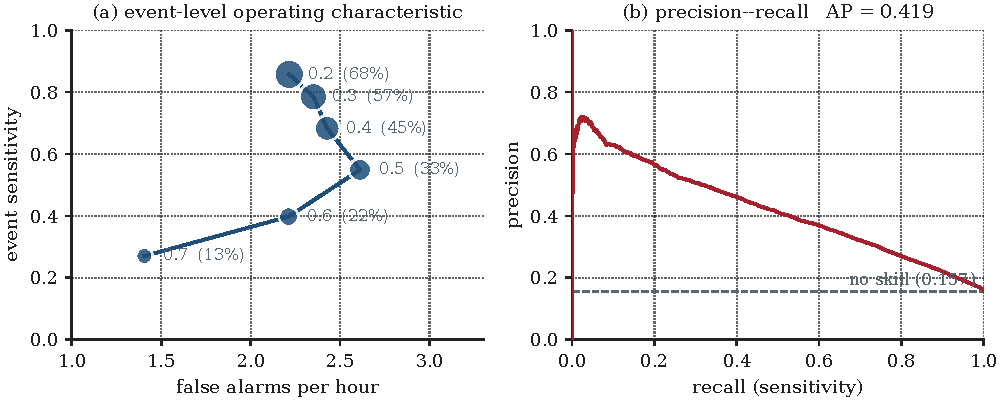
\includegraphics[width=\columnwidth]{figures/fig_roc_pr.pdf}
\caption{Respiratory-event detection, pooled over the ten patient-independent test
folds. \textbf{(a)} Event-level operating characteristic. Each point is a decision
threshold, labelled and sized by the fraction of all epochs it flags.
\textbf{(b)} Precision--recall; the dashed line is the $0.157$ event prevalence, the
no-skill floor.}
\label{fig:rocpr}
\end{figure}

\begin{table}[t]
\caption{Respiratory-event detection, ten-fold patient-independent. \textit{(a)}
Detectors on the same folds; the classical baselines read the $14$ descriptors, MM-Net the
raw signal. $^{\S}$~Raw-signal CNN--BiLSTM detectors trained end to end on the waveforms,
the first on the input configuration of~\cite{nassi2022effortbelt}; single seed, ten
folds. Chance
average precision is the $0.157$ prevalence. \textit{(b)} AUC by event
type, $96$ annotated patients. Best per column in \textbf{bold}.}
\label{tab:resp}
\centering
\small
\begin{tabular}{lcc}
\toprule
\multicolumn{3}{l}{\textit{(a) Detection method}}\\
\midrule
Method & AUC\,$\uparrow$ & AP\,$\uparrow$ \\
\midrule
Desaturation rule    & 0.596 & 0.214 \\
Logistic regression  & 0.582 & 0.193 \\
Gradient boosting    & 0.670 & 0.290 \\
Raw effort belt$^{\S}$~\cite{nassi2022effortbelt} & 0.605 & 0.240 \\
Raw seven channels$^{\S}$ & 0.735 & 0.361 \\
MM-Net (proposed)    & \textbf{0.782} & \textbf{0.419} \\
\bottomrule
\end{tabular}

\vspace{4pt}
\begin{tabular}{lcc}
\toprule
\multicolumn{3}{l}{\textit{(b) MM-Net AUC by event type}}\\
\midrule
Event type & Positive epochs & AUC\,$\uparrow$ \\
\midrule
Hypopnea    & 11{,}605 & 0.748 \\
Obstructive & 1{,}661  & 0.898 \\
Central     & 831      & \textbf{0.935} \\
\bottomrule
\end{tabular}
\end{table}

\subsection{Clinical Validation against AHI and Severity}
Aggregating the per-epoch respiratory probability into a per-patient burden and correlating it
with the clinical apnea-hypopnea index (AHI) from the metadata gives a significant positive
association (Spearman $\rho=0.491$, $p<0.001$, $n=99$, the twelve recordings with an
incomplete cardiorespiratory montage scored with those channels zero-filled;
Fig.~\ref{fig:ahi}), so the model's output tracks a
clinician's summary measure beyond an epoch-level score. Staging, in turn, degrades as
sleep-disordered breathing worsens: accuracy falls from $0.769$ in patients with a normal AHI to
$0.719$ in the severe group (Table~\ref{tab:severity}). The pathology that motivates the second output also makes the first
harder, which is the clinical reality of this cohort.

The association is statistically significant but modest in magnitude.
Three mechanisms plausibly limit it, and each is a property of the formulation rather
than of the model. First, mean per-epoch probability is a poor estimator of an hourly event
rate: a $30$-second epoch holding one hypopnea and one holding three both contribute a
single positive, so the aggregate compresses exactly the variation the index is built from.
Second, the clinical index is normalised by total sleep time, whereas our burden averages
over every scored epoch including wake, and the two denominators diverge most in the
patients with the most fragmented sleep, which in this cohort is the severe group.
Third, the AHI itself carries substantial night-to-night variability, so a single-night
reference sets a ceiling on any correlation with it. We therefore read $\rho=0.491$ as
evidence that the read-out tracks severity at the group level, without claiming that it
estimates an index.

\begin{figure}[t]
\centering
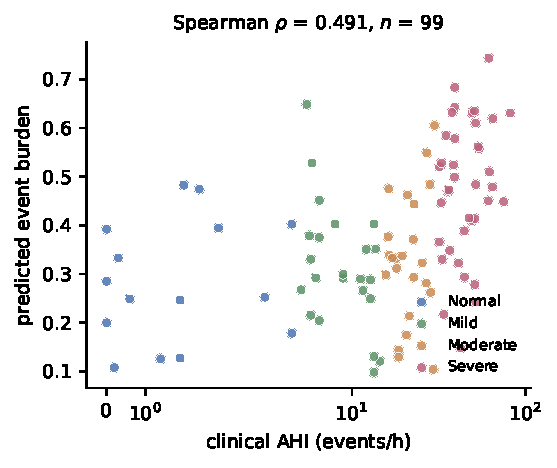
\includegraphics[width=0.86\columnwidth]{figures/fig_ahi.pdf}
\caption{Predicted per-patient event burden (mean respiratory probability) against the clinical
apnea-hypopnea index, coloured by AASM severity band. The positive association (Spearman
$\rho=0.491$, $n=99$) shows the model's output tracks a clinician's summary measure.}
\label{fig:ahi}
\end{figure}

\begin{table}[t]
\caption{Sleep-staging accuracy by sleep-disordered-breathing severity (AASM AHI bands),
ten-fold patient-independent; mean\,$\pm$\,SD across patients ($N=99$). Staging degrades
monotonically as severity rises (Jonckheere--Terpstra test for a decreasing trend across the
four ordered bands, one-sided $p=0.030$; Spearman correlation of per-patient accuracy with
AHI $\rho=-0.18$, $p=0.074$). Wake share is not correlated with AHI ($\rho=-0.03$).}
\label{tab:severity}
\centering
\small
\begin{tabular}{lccc}
\toprule
AHI band & AHI (events/h) & Patients & Staging acc\,$\uparrow$ \\
\midrule
Normal   & $<5$       & 15 & $0.769 \pm 0.049$ \\
Mild     & $5$--$15$  & 23 & $0.747 \pm 0.069$ \\
Moderate & $15$--$30$ & 23 & $0.722 \pm 0.088$ \\
Severe   & $\geq 30$  & 38 & $0.719 \pm 0.100$ \\
\bottomrule
\end{tabular}
\end{table}

\subsection{Permutation Importance: a Second, Independent Attribution}
The ablation grid establishes what the model \emph{needs}: remove a modality, retrain, and
observe which head suffers. A complementary question is what a \emph{trained} model actually
uses. We therefore permute each modality's features across epochs at inference time, so the
channel is still present but no longer aligned to the epoch it describes, and measure the
drop, averaged over three shuffles and the ten fold models.

The two methods can disagree, because a model may need a channel during training yet weight it
lightly afterwards. On staging they do not: permuting the neural features costs $0.284$ staging
accuracy against $0.030$ for the ocular and $0.006$ for the muscle channel, the same ordering
the ablation gives, and the rank correlation between the two attributions is $\rho=0.833$
($p=0.010$).

On the respiratory head the agreement is narrower, and we report the two attributions
separately. Both methods place respiratory effort first by a wide
margin: $0.038$ AUC under retraining, $0.071$ under permutation, in each case well clear of
the runner-up. The remaining four cardiorespiratory channels, however, have retraining effects
that are not distinguishable from zero, so their rank order carries no signal there and the
correlation over the five is correspondingly uninformative ($\rho=0.381$, $p=0.35$).

Permutation separates them where retraining cannot. Each fold records its own baseline
AUC and its AUC after shuffling, so the drop is a within-fold quantity and can be tested
directly. Every channel's drop is distinguishable from zero (one-sample on ten per-fold drops,
Holm across the eight channels): effort $0.071$ ($p<10^{-4}$), airflow $0.027$ ($p=0.0005$),
SpO$_2$ $0.016$ ($p=0.0002$), pulse/HRV $0.012$ ($p=0.004$), and the remainder below $0.006$.
Significance here is not importance. The magnitudes span a factor of $32$, and what the test
establishes is that the \emph{ordering} is real. That ordering is the substantive
result: the three channels the model relies on most, effort, airflow and SpO$_2$,
are exactly the three the AASM definition of a respiratory event is written in, and they are
one to two orders above the cardiac and muscle channels.

The two experiments answer different questions, so the divergence is informative. Retraining without a channel measures whether it is \emph{irreplaceable}, and
the network compensates by re-learning the signal from its correlates; permutation holds the
fitted model still and measures what it \emph{uses}. SpO$_2$ is the clearest case: retraining
without it costs $0.002$ AUC, shuffling it under the fitted model costs $0.016$. A channel can
be heavily used and still be replaceable. The claim the comparison supports is therefore the
one that matters physiologically: two attributions sharing no machinery, one applied to
retrained models and one to fixed ones, independently identify effort as the dominant
respiratory cue.

\subsection{Data Efficiency and the Limits of Cohort Size}
\label{sec:curve}
Staging accuracy on this corpus remains near $0.72$--$0.75$ across the model families
evaluated here. Whether that reflects the architecture or the cohort is testable: retrain the
identical model on a shrinking fraction of the \emph{training patients}, always evaluating on
the full held-out fold (Fig.~\ref{fig:curve}). Subsampling is by patient,
because epochs within a patient are heavily correlated.

The two heads answer differently. Staging accuracy rises $0.701 \rightarrow 0.721 \rightarrow
0.726 \rightarrow 0.735$ as training patients go from $20$ to $79$, with marginal gains of
$+0.020$, $+0.005$ and $+0.009$, all under half a fold standard deviation and flattening.
Respiratory AUC over the same range rises $0.732 \rightarrow 0.750 \rightarrow 0.752
\rightarrow 0.785$, and its \emph{largest} increment is the final one, $+0.033$, close to a
full fold standard deviation, and steeper than any earlier step. This curve is a single seed
on a fixed held-out set, so its endpoint differs slightly from the three-seed headline figures
($\mmAcc$ and $\mmAuc$); the shape is what this curve is here to show. Staging has stopped
responding to added patients at this sample size; respiratory detection has not, and its final
increment is consistent across folds ($+0.033$ AUC from $59$ to $79$ patients, ten of ten
folds, Wilcoxon $p=0.002$). We draw the
narrower conclusion the data support: over the range we can test, more patients of this kind
would improve breathing detection and would not appreciably improve staging. That is a
statement about the returns to cohort size for these methods. It is not a measurement of an
irreducible error rate, which fewer than a hundred patients and a finite set of architectures
cannot establish. The final model also exceeds
the feature-only configuration at the full training-set size, so its advantage is not an
artefact of the full sample.

\begin{figure}[t]
\centering
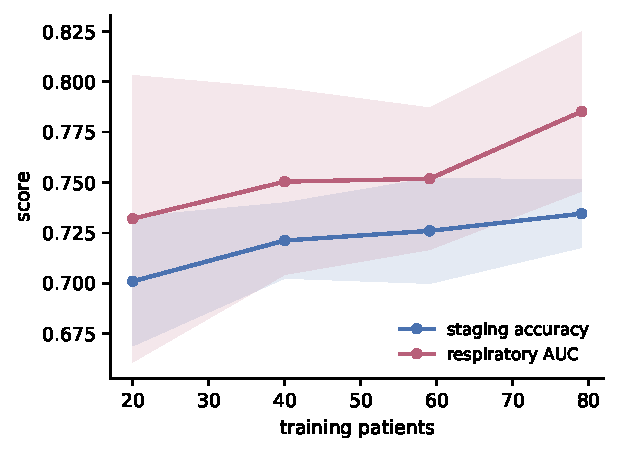
\includegraphics[width=0.86\columnwidth]{figures/fig_learning_curve.pdf}
\caption{Learning curve over training-patient fraction, ten-fold patient-independent, error
bars one standard deviation across folds. Staging (blue) flattens by $59$ patients; respiratory
detection is still rising at $79$. Bands are $\pm$ one standard deviation
across folds.}
\label{fig:curve}
\end{figure}

\subsection{Healthy-Trained Models Applied to the Injured Brain}
\label{sec:domaingap}
Table~\ref{tab:bench} retrains published architectures \emph{on} iSLEEPS. A different and
harder question is what happens when a model built for healthy sleep is applied to this cohort
as published. The three architectures are our own: a four-channel CNN, the same
CNN with a BiLSTM over epochs, and StagingSeqNet, a deeper convolutional-recurrent stager we
built for this comparison. Naming them matters only in that none is a weak straw man; each
reaches $0.81$ to $0.86$ on the healthy corpus it was trained on. We trained them on the
Sleep-EDF Cassette subset and applied each to all
$99$ iSLEEPS patients zero-shot, with no adaptation of any kind. This is the middle block of
Table~\ref{tab:bench}, set against the same architectures retrained on this cohort.

The result is not a degradation but a collapse. All three stage healthy sleep competently,
$0.806$ to $0.855$ accuracy and $\kappa$ $0.73$ to $0.81$; on stroke the same checkpoints reach
$0.306$ to $0.312$ with $\kappa$ $0.09$ to $0.13$, which is close to chance for a five-class
problem with this prior. The failure mode is more informative than the headline. Wake takes
$62$ to $79\%$ of predicted stroke epochs against a true $26.7\%$, while N2 falls to between
$1$ and $5\%$ of predictions on the stage that is $42.3\%$ of the data, and N2 recall on the
worst of the three is $0.015$. These models do not lose accuracy
gracefully; they stop recognising sleep architecture at all.

The control is what makes this interpretable. A healthy-trained stager scoring $0.31$
on iSLEEPS is evidence of a cohort effect only if the same checkpoint, through the same
preprocessing, scores properly on healthy sleep; otherwise a broken input pipeline and a
genuine domain gap produce identical numbers. Run through our pipeline on held-out Sleep-EDF
recordings, the strongest checkpoint holds at $0.8682$ ($0.8667 \pm 0.0415$ per recording), so
the pipeline is correct and the collapse belongs to the cohort.

These results should be interpreted together with the difference in EEG montage between the two datasets. Sleep-EDF uses Fpz-Cz and Pz-Oz, whereas iSLEEPS uses C4 and O2. The zero-shot performance gap may therefore reflect both the change in cohort and the change in montage. Deep models trained \emph{on} iSLEEPS with the matched montage reach $0.60$--$0.72$ (upper block), and the same architectures lose $0.12$ to $0.15$
accuracy between healthy sleep and stroke under a common protocol; healthy-trained and
zero-shot, with the montage shift included, the cost is $0.56$. The claim is bounded by those two figures together.

The same argument run in reverse. Every figure above concerns other
architectures, which leaves the obvious question unanswered: whether $\mmAcc$ is low
because the cohort is hard or because the proposed model is weak. So we cross-validated it
on healthy sleep, ten-fold and subject-independent over the $21$ Sleep-EDF subjects, using the
neural branch alone since that corpus carries none of the cardiorespiratory channels we read. It reaches
$0.856 \pm 0.027$ accuracy with $\kappa$ $0.800$ (final row of Table~\ref{tab:bench}).
That places it among the healthy-sleep stagers in the middle block,
against $0.741$ for the identical architecture on stroke. The $0.115$ difference is what
the cohort costs a model that is demonstrably capable of more, which is a stronger
statement than any comparison against other people's architectures can make.

The cohort does not cost every architecture equally. Ten retrained baselines carry a
healthy-sleep score produced by the same code under the same protocol, so the table shows how
much each model loses in the crossing. AttnSleep falls $0.117$ ($0.833 \to 0.716$),
1D-ResNet-SE-LSTM $0.124$, SE-ResNet-18\,+\,BiLSTM $0.133$, SleepTransformer $0.140$, AT-BiLSTM $0.143$, U-Time $0.145$,
TinySleepNet $0.148$ and Micro SleepNet $0.153$; DeepSleepNet ($0.154$) and the CNN\,+\,BiLSTM
($0.136$) read two EEG derivations on Sleep-EDF and four on iSLEEPS. The proposed model falls
$0.115$ ($0.856 \to 0.741$), the smallest loss in the table, with AttnSleep closest. We report
this as an observation. These differences do not support a significance test, and the
comparison is between systems rather than a controlled ablation, since the proposed rows read
engineered features and a frozen embedding while most baselines read a single raw channel. The
direction is nonetheless the one the rest of the paper predicts: a representation that
encodes sleep physiology explicitly survives a disordered cortex better than one a network
must discover for itself from fewer than a hundred patients.

% Folds are split by subject, not by recording, because Sleep-EDF Cassette records
% each subject on two nights; splitting on filenames would place the same person on both
% sides of a fold.
We split the folds at the subject level. Sleep-EDF Cassette records each subject on two nights. Splitting by recording could therefore place the same person in both the training and test folds.




\subsection{Stream Representations}
\label{sec:repr}
The architecture uses engineered features together with a frozen self-supervised embedding for the neural stream and a learned convolutional encoder over the raw cardiorespiratory signal. Both representation choices were evaluated experimentally before selection. Each family below holds every other hyperparameter fixed and varies one thing, over
the same three seeds and ten patient-independent folds, with Holm correction within the
family and every test on the ten fold-means.

The engineered cardiorespiratory representation appears to be the principal limitation, and
part of the gap can be recovered without additional input information. Each block of Table~\ref{tab:repr} holds the other stream at its baseline, so no single
row there is the full model, and the two baselines differ: the cardiorespiratory block runs
the $188$ neural descriptors without the pretrained embedding, while the neural block runs the
$14$ engineered cardiorespiratory descriptors. That is why the two blocks report different
respiratory AUC for what both call an engineered-feature reference ($0.698$ against $0.685$),
and why the adopted cardiorespiratory row reads $0.740$ staging accuracy against the headline
$\mmAcc$, which adds the pretrained embedding on top of it. The upper block replaces the $14$ engineered cardiorespiratory features
with progressively richer representations of the same underlying signal. Every step is
significant, and the ordering identifies where the limitation lies. A \emph{random} nonlinear expansion of the same
$14$ numbers recovers $0.018$ AUC, which is obtained without additional input information and with only more
capacity to read what was already computed, which says the summary features leave nonlinear
structure unrepresented. A random linear projection of the raw waveform adds a further $0.016$,
so part of what the features discard is recoverable without learning anything. The learned
convolutional encoder reaches $0.782$, $0.084$ above the engineered features.

These results identify the representation of the cardiorespiratory stream, rather than the detector above it, as the factor limiting the respiratory read-out; the detector is held fixed throughout. These results
attribute the improvement to the change in representation rather than to the specific encoder
architecture.

The same search also evaluated a general time-series foundation model,
MOMENT~\cite{goswami2024moment}, as a frozen cardiorespiratory encoder. With its pretrained
weights it reaches $0.808$ respiratory AUC, and with randomly initialised weights $0.795$,
both above the learned encoder ($0.782$) and both at comparable staging accuracy
(Table~\ref{tab:repr}). The randomly initialised version is the encoder most often selected by
the nested procedure of Section~\ref{sec:nested}. The learned convolutional encoder was
retained for the final model because it has $0.155$ million trainable parameters against
$341$ million frozen ones, is trained end to end with the rest of the network, and requires
no external model; the respiratory results of this paper should therefore be read as
obtainable with several encoders, the learned one being the smallest of them.

On the neural side a pretrained encoder does not replace expert features, but does
add to them. The lower block of Table~\ref{tab:repr} varies the neural representation with the
cardiorespiratory stream held at the engineered features. Used alone, the frozen encoder is
significantly \emph{worse} than the $188$ features ($-0.029$, Holm $p=0.008$): pretraining on
healthy scalp EEG does not by itself substitute for physiology chosen for this task.
Concatenated with the features it adds $+0.008$ accuracy (Holm $p=0.006$), and a second
pretrained encoder on top of the first adds nothing further ($-0.004$, $p=0.56$).

These results support a narrow interpretation: expert physiology and
self-supervised pretraining encode partly different information, so their union beats either
alone; but the complementarity saturates after one pretrained encoder, so this is not a
general argument for stacking foundation models.

\begin{table*}[t]
\caption{What each stream should be represented as. One factor varies per block,
everything else held fixed; cells are mean $\pm$ SD over thirty fold-values. \textup{\unboldmath$\Delta$} and
Holm $p$ are against each block's engineered-feature baseline, the latter on the ten
fold-means. ``adopted'' marks the choice carried into the final model.
$^{\dagger}$~MOMENT-1-large~\cite{goswami2024moment}, $341$\,M parameters, frozen, with its
pretrained weights or randomly initialised, applied to the seven-channel epoch resampled to
$512$ samples, with its embedding appended to the $14$ descriptors; the Holm family of the
cardiorespiratory block comprises its five comparisons.}
\label{tab:repr}
\centering
\begin{tabular*}{\textwidth}{@{\extracolsep{\fill}} l l c c c c @{}}
\toprule
Representation & Variant & Resp.\ AUC\,$\uparrow$ & Staging acc\,$\uparrow$ & $\Delta$ & Holm $p$ \\
\midrule
\multirow{6}{*}{\emph{Cardiorespiratory}}
 & $14$ engineered features               & $0.698 \pm 0.051$ & $0.736 \pm 0.014$ & ---      & ---      \\
 & random nonlinear expansion of the $14$ & $0.715 \pm 0.047$ & $0.737 \pm 0.018$ & $+0.018$ & $0.012$   \\
 & random linear projection of raw signal & $0.731 \pm 0.044$ & $0.735 \pm 0.021$ & $+0.034$ & $0.012$   \\
 & learned CNN, $0.155$\,M (adopted)      & $0.782 \pm 0.040$ & $0.740 \pm 0.019$ & $+0.084$ & $\mathbf{0.010}$ \\
 & random-init.\ time-series encoder$^{\dagger}$ & $0.795 \pm 0.045$ & $0.737 \pm 0.017$ & $+0.097$ & $0.010$ \\
 & pretrained time-series encoder$^{\dagger}$    & $\mathbf{0.808 \pm 0.042}$ & $0.734 \pm 0.018$ & $+0.110$ & $0.010$ \\
\midrule
\multirow{4}{*}{\emph{Neural}}
 & $188$ engineered features            & $0.685 \pm 0.041$ & $0.741 \pm 0.016$ & ---      & ---      \\
 & frozen pretrained encoder alone      & $0.681 \pm 0.033$ & $0.712 \pm 0.033$ & $-0.029$ & $0.008$   \\
 & features $+$ pretrained (adopted)    & $0.690 \pm 0.037$ & $\mathbf{0.749 \pm 0.018}$ & $+0.008$ & $\mathbf{0.006}$ \\
 & features $+$ two pretrained encoders & $0.684 \pm 0.043$ & $0.745 \pm 0.018$ & $+0.004$ & $0.23$   \\
\bottomrule
\end{tabular*}
\end{table*}

\subsection{The Two Loss Constants}
\label{sec:losssens}
Two constants in Section~\ref{sec:method} were fixed by argument:
the task balance $\lambda=1$ and the positive weight $\pi=n_-/n_+$, which is $5.35$ on this
corpus. Equal coefficients do not make equal influence, since the two terms differ in scale
and curvature, so $\lambda=1$ is a claim about arithmetic. We therefore
swept each with everything else at the published setting, three seeds by ten folds per value,
and evaluate both heads at every point, since the relevant outcome is not a lower value on
one head but a trade-off between them.

No trade-off is observed, and the effect of either constant is small. Across $\lambda$ from
$0.25$ to $4$
staging accuracy spans $0.003$ and respiratory AUC $0.018$, and across $\pi$ from $1$ to $11$
they span $0.003$ and $0.007$; the fold-to-fold standard deviations are $0.019$ and $0.038$.
Both heads attain their maximum at the same $\lambda$, which is inconsistent with a
compromise setting: were $\lambda=1$ balancing one task against the other, the two curves
would peak on opposite sides of it.

Neither published value is the maximum of those tested. Staging is highest at $\lambda=2$
($0.7403$) and at $\pi=11$ ($0.7422$), and respiratory AUC at $\lambda=2$ ($0.7840$) and
$\pi=8$ ($0.7846$). All of these margins are below a fifth of a fold standard deviation, so
the sweep does not identify better settings; it establishes that the objective is insensitive
to both constants across the range examined, and that fixing them a priori has no measurable
cost on this corpus.

\subsection{Calibration and Selective Prediction}
A clinical reader needs to know not only how often the model is right but whether it knows when
it is likely to be wrong. Two measurements answer that, both computed on held-out epochs with
the raw posteriors before HMM smoothing.

% The model is \emph{overconfident}: expected calibration error, over ten equal-width confidence
% bins weighted by occupancy and ignoring bins holding fewer than fifty epochs, is $0.076$, and
% the gap runs one way in every bin: epochs it scores above $0.9$ are correct $88\%$ of the time.
% Stated confidences should therefore be read as ordered, not as probabilities, which is the
% displacement Section~\ref{sec:method} derives arriving in the measurement.

The model shows some overconfidence. Its expected calibration error is $0.076$. We calculate this value using ten equal-width confidence bins weighted by occupancy. Bins containing fewer than fifty epochs are excluded from the calculation. The same calibration pattern appears across the confidence bins. For example, epochs with confidence scores above $0.9$ are correct $88\%$ of the time. The confidence scores are therefore most useful for ordering predictions by certainty. Section~\ref{sec:method} explains why their numerical values differ from calibrated probabilities.




Ranking, however, is what abstention needs. Applying split-conformal prediction with the
fold's validation patients as the calibration set gives empirical coverage that tracks the
target closely ($0.894$ at a $0.90$ target, $0.943$ at $0.95$). At $\alpha=0.10$ the model
returns a single stage for $45.8\%$ of epochs and is correct on $86.9\%$ of those, against
$59.1\%$ on the epochs where it returns a larger set. The abstention is therefore selecting the
genuinely hard epochs, and it concentrates where a scorer would
expect: N1 receives a singleton set only $19\%$ of the time, the lowest of any stage and the
one human scorers agree on least.

Two caveats attach to the coverage figures rather than to the abstention behaviour. The
calibration patients are the same patients that stopped training, so their labels have already
influenced which checkpoint was kept and they are not the independent calibration sample
split-conformal theory assumes; the coverage we report is therefore empirical and carries no
guarantee. And epochs within a night are strongly dependent, so the exchangeable unit is
closer to the patient than to the epoch, which makes these marginal rates across pooled
epochs and not coverage for a new patient or within any one stage. A calibration split
disjoint from early stopping would settle both, and we did not run one.

\subsection{External Validation on Two Independent Corpora}
\label{sec:external}
Ten-fold cross-validation is patient-independent but remains within one corpus, one centre
and one acquisition protocol. We therefore trained a single model on all $99$ iSLEEPS
patients and evaluated it, unchanged, on two public corpora with no dataset-specific
tuning: no fine-tuning, no threshold search, no re-fitted model or decision threshold (per-recording feature standardisation is applied, as in training), and hidden-Markov
transitions estimated from iSLEEPS alone (Table~\ref{tab:ext}).

The two corpora test different things. \textbf{Sleep-EDF}~\cite{kemp2000sleepedf}
is healthy sleep recorded on a frontal montage (Fpz-Cz, Pz-Oz). Its Cassette recordings carry
an oronasal airflow trace at $1$\,Hz but no ECG, effort belts or oximetry, and no scored
respiratory events, so six of our seven cardiorespiratory inputs are absent and the
respiratory head cannot be scored there; it tests the staging head across both a cohort shift
and a montage shift.
\textbf{ISRUC-Sleep}~\cite{khalighi2016isruc} is a sleep-disorders cohort recorded on the
same central and occipital derivations we use (C4, C3, O2, O1 against the contralateral
mastoid), with SpO$_2$, airflow, effort and ECG, and with obstructive, central and mixed
apneas and hypopneas scored, so it tests the staging head \emph{without} a montage
confound and provides the only external test of the respiratory head. Because Sleep-EDF
carries almost none of those channels, that branch is fed zeros there. Zeroing an input that the network was trained to use creates a train/test mismatch, so we do not treat this as an ablation. To address this, we also trained a separate model with the corresponding branch zeroed throughout training. This model reaches $0.774$ accuracy, compared with $0.794$ for the full model. These are two separate procedures, and neither provides an upper or lower bound on the other. We therefore report both results and do not draw conclusions from the higher value alone. The mismatched run could be gaining from batch-normalisation statistics that never
saw zeros, in which case $0.774$ is the more defensible number, and a reader who prefers it
loses nothing in our argument: both sit above the in-domain $\mmAcc$. Sleep-EDF also
differs from iSLEEPS in montage, so its transfer figure is a lower bound and not a clean
estimate. ISRUC records each
subject twice; respiratory-event prevalence is $10.1\%$ on the first night and $2.4\%$ on
the second, so we report the two separately; pooling would merge a difference that has
nothing to do with the model.

The respiratory read-out transfers. On ISRUC night one the model reaches
$0.780$ AUC, and it does so handicapped, because ISRUC provides no pulse channel and no
separate effort trace, leaving two of the seven cardiorespiratory inputs zero-filled. A
detector that had latched onto one centre's equipment would not survive that; this one does.
The comparison requires matched estimators, which we state before giving the two numbers. The external figure is pooled over all epochs of the
night, because per-recording AUC is unusable on this corpus: event prevalence ranges from
$0\%$ to $22\%$ across the sixteen recordings, and a night with a handful of positive epochs
returns an estimate whose sampling variance swamps any difference between models, while a
night with none leaves AUC undefined. The in-domain headline $\mmAuc$ is a ten-fold mean.
Pooled in-domain, the like-for-like quantity, is $0.777$. The external result therefore
sits within $0.003$ of the in-domain one on either estimator, and nothing in the claim rests
on which is chosen. Night two falls to $0.723$. Its event prevalence is much lower ($2.4\%$
against $10.1\%$), which does not by itself depress AUC, since ranking is insensitive to the
mix; what the scarcity of positives does is widen the uncertainty on that night's estimate,
so we read the two nights as one imprecise result.

Staging moves in opposite directions on the two corpora, for reasons the data
identify. On Sleep-EDF the model \emph{gains} $0.084$ of $\kappa$ over its in-domain
score. A representation that had memorised corpus-specific artefacts would degrade out of
corpus, so the straightforward reading is that the features are physiological and that the
accuracy range reported throughout this paper is associated with \emph{stroke sleep} rather
than with the model. The learning curve supports the same interpretation
(Section~\ref{sec:curve}) by a
different route. On ISRUC staging falls by $0.090$ accuracy, and the class mix explains
much of it: ISRUC carries $15.6\%$ N1 against iSLEEPS' $10.2\%$ and Sleep-EDF's $6.6\%$,
and N1 is the weakest stage in every cohort we have measured (recall $0.168$ on ISRUC,
$0.294$ on Sleep-EDF, and the lowest per-class F1 in-domain).

Montage does not appear to govern N3 transfer. N3 recall is $0.841$ on Sleep-EDF, whose
frontal montage differs from ours, with $12.7\%$ of N3 read as N2, and $0.630$ on ISRUC, whose
derivations match ours, with $34.8\%$. With one external pass per corpus and eight ISRUC
subjects, this pattern is reported without a causal attribution.

Two limitations qualify this analysis. Accuracy across cohorts with different class balance is
not directly comparable, which is why $\kappa$ is reported alongside. And ISRUC contributes
only eight subjects. Per-recording accuracy spans $0.458$--$0.748$, so the ISRUC
figures in Table~\ref{tab:ext} are quoted to three decimals for consistency with the rest of
the paper and should be read to two; per-recording
respiratory AUC spans $0.515$--$0.848$, with the widest uncertainty on the nights carrying
fewest scored events.

\begin{table}[t]
\caption{External validation, zero-shot: one model trained on all $99$ iSLEEPS
patients, no dataset-specific tuning. In-domain figures are ten-fold means. Sleep-EDF carries
no scored respiratory events and almost none of our cardiorespiratory channels, so the
respiratory head is unscored there; the two ISRUC nights
differ in event prevalence and are reported separately.}
\label{tab:ext}
\centering
\setlength{\tabcolsep}{4pt}
\resizebox{\columnwidth}{!}{%
\begin{tabular}{llcccc}
\toprule
Corpus & Cohort & Rec. & Acc\,$\uparrow$ & $\kappa$\,$\uparrow$ & Resp.\ AUC\,$\uparrow$ \\
\midrule
iSLEEPS (in-domain)   & stroke        & 99 & $\mmAcc$ & $\mmK$ & $\mmAuc$ \\
\midrule
Sleep-EDF             & healthy       & 40 & $\mathbf{0.794}$ & $\mathbf{0.718}$ & --- \\
ISRUC, night 1        & sleep-disord. &  8 & $0.649$ & $0.536$ & $\mathbf{0.780}$ \\
ISRUC, night 2        & sleep-disord. &  8 & $0.575$ & $0.426$ & $0.723$ \\
\bottomrule
\end{tabular}}
\end{table}

\subsection{Model Complexity and Capability}
Table~\ref{tab:cost} sets the proposed model beside representative alternatives on size and
capability. At $2.76$\,M trainable parameters the model is an order of magnitude
smaller than DeepSleepNet ($\sim$$21$\,M) and the corpus's own CNN-ResNet18 ($\sim$$11$\,M),
and comparable to SleepTransformer, so size is not where it wins. It delivers both a
competitive stage and a respiratory read-out from one pass over the recording, and none of
the staging-only models, at any size, can supply the second output.

\begin{table}[t]
\caption{Model size and clinical capability. The proposed model is mid-sized and is the only
one that produces both a stage and a respiratory-event label at competitive staging accuracy;
the raw multimodal CNN produces both but stages at $0.677$.}
\label{tab:cost}
\centering
\setlength{\tabcolsep}{4pt}
\begin{tabular}{lccc}
\toprule
Model & Input & Params\,$\downarrow$ & Outputs \\
\midrule
CNN-ResNet18~\cite{bose2026gap}           & 1\,EEG      & $\sim$11\,M & stage \\
DeepSleepNet~\cite{supratak2017deepsleepnet} & 1\,EEG   & $\sim$21\,M & stage \\
Raw multimodal CNN                        & 14\,ch      & 0.95\,M     & stage + apnea \\
\textbf{MM-Net (proposed)}                & 7\,ch feat $+$ raw & \textbf{2.76\,M} & \textbf{stage + apnea} \\
\bottomrule
\end{tabular}
\end{table}

%=====================================================================
\section{Discussion}
\label{sec:discussion}

This study shows that sleep staging and respiratory-event prediction can be
integrated within a single model for subacute ischemic-stroke PSG while
preserving a clear physiological organization between the two tasks. MM-Net
reaches $0.739$ sleep-staging accuracy ($\kappa=0.634$) together with a
respiratory-event AUC of $0.782$. The more informative result comes from the
controlled interventions: neural information carries most of the discriminative
structure for sleep staging, whereas cardiorespiratory information carries the
respiratory task. Joint optimization then provides a smaller but consistent
additional benefit across the two outputs. The resulting model therefore
combines two clinically related analyses through shared temporal context while
retaining task-specific physiological dependence.

This organization extends previous joint sleep-analysis work to a
stroke-specific setting. Huttunen \emph{et al.}
~\cite{huttunen2023simultaneous} demonstrated simultaneous sleep staging and
respiratory-event scoring in a large suspected-obstructive-sleep-apnea cohort.
Under the common iSLEEPS evaluation used here, their architecture reaches
$0.599$ staging accuracy and $0.710$ respiratory AUC, compared with $0.739$ and
$0.782$ for MM-Net. The difference is important in the context of the present
population, where the available montage, cohort size, neural physiology, and
respiratory annotation differ from those of conventional sleep-apnea studies.
The results indicate that joint PSG analysis in stroke benefits from
representations and signal organization adapted to the characteristics of the
target cohort.

The modality-ablation experiments provide the strongest evidence for this
interpretation. Removing the cardiorespiratory stream reduces respiratory AUC
to $0.654$ while leaving staging essentially unchanged. Removing the neural
stream produces the complementary response, reducing staging accuracy to
$0.680$ while respiratory discrimination is largely preserved. These
interventions identify a strong task-specific dependence within the trained
model. Cortical, ocular, and muscular information provides the principal basis
for distinguishing sleep stages, while respiratory and cardiovascular signals
provide the principal basis for identifying respiratory disturbance. The
shared temporal decoder therefore connects two tasks whose immediate
physiological evidence remains largely distinct.

The structure within the cardiorespiratory stream further clarifies how the
respiratory output is formed. Respiratory effort is the strongest individual
contributor, with its removal producing the largest channel-specific loss.
Removing the complete cardiorespiratory stream, however, causes a much larger
reduction than removing any single signal. This pattern indicates that
respiratory information is distributed across partially overlapping
measurements of breathing mechanics, oxygenation, and cardiovascular response.
The airflow intervention gives this interpretation additional support:
respiratory AUC remains $0.778$ after airflow is removed, compared with $0.782$
for the complete model. The respiratory decision therefore remains supported by
complementary physiological information even when the primary airflow signal is
absent. This distributed dependence is also consistent with the stability of
respiratory performance in recordings with incomplete cardiorespiratory
montages.

The representation experiments identify where much of the modeling gain
originates. Fourteen engineered cardiorespiratory descriptors reach an AUC of
$0.698$, while progressively richer representations of the same physiological
signals recover additional performance, culminating in $0.782$ for the learned
raw-signal encoder. The nested model-selection experiment supports the same
interpretation from a separate direction: several higher-capacity
cardiorespiratory representations perform competitively across the outer
folds. The important design principle is therefore the preservation of richer
temporal information from the underlying respiratory and cardiac waveforms.
CardioCNN provides an effective implementation of this principle in MM-Net,
while the broader gain is associated with representation quality rather than a
single encoder configuration.

The neural stream follows a complementary pattern. Engineered descriptors form
a strong standalone representation for sleep staging, while the frozen
pretrained EEG representation adds information when combined with them. The
engineered features reach $0.741$ staging accuracy in the controlled
representation experiment, and their combination with the pretrained
representation reaches $0.749$. This result suggests that sleep-specific
physiological descriptors and large-scale EEG pretraining encode partly
different aspects of the neural signal. The former contributes structure
selected explicitly for sleep physiology, while the latter contributes
representations learned from broader EEG data~\cite{labram2024}. Their
combination is well matched to the present setting, where the supervised stroke
cohort is modest in size and fully end-to-end representation learning would
place a greater burden on the available data.

The matched single-task experiments show how these specialized streams benefit
from joint temporal learning. Joint optimization raises staging accuracy from
$0.733$ to $0.739$ and respiratory AUC from $0.774$ to $0.782$, with the same
direction observed across most patient folds. The effect is consistent with the
structure of the problem: sleep stage and respiratory disturbance arise from
different immediate physiological measurements, yet both evolve within the
same overnight sequence. Shared temporal modeling can therefore exploit common
context while the modality-specific encoders preserve the information required
by each task. The fusion experiments reinforce this interpretation. Simple
concatenation is sufficient to combine the streams, and the aligned
cardiorespiratory pathway to the respiratory head provides an additional
task-specific contribution. The performance of the model is consequently driven
primarily by the quality and temporal alignment of the physiological
representations rather than by fusion complexity.

The staging experiments also reveal the importance of evaluating sleep models
within the population in which they will be used. Deep architectures retrained
on iSLEEPS reach approximately $0.62$--$0.72$ accuracy, while MM-Net reaches
$0.739$ with a macro-F1 of $0.670$. The healthy-to-stroke transfer experiment
shows an even larger shift: models achieving approximately $0.81$--$0.86$
accuracy on Sleep-EDF reach only about $0.31$ when applied directly to iSLEEPS
without adaptation. Because population, montage, and acquisition conditions
change together, this experiment is most appropriately interpreted as evidence
of a substantial domain shift between conventional healthy-sleep data and
subacute stroke PSG. The same MM-Net neural architecture reaches $0.856$
accuracy under patient-independent evaluation on Sleep-EDF and approximately
$0.74$ within the stroke cohort, further illustrating how strongly the observed
performance depends on the target population.

The external evaluations provide complementary evidence that the learned
representations remain useful beyond the development cohort. The iSLEEPS-trained
model reaches $0.794$ staging accuracy on Sleep-EDF, while ISRUC-Sleep provides
an independent test under a different sleep-disorder population and signal
configuration. Respiratory AUC reaches $0.780$ and $0.723$ on the two ISRUC
nights despite unavailable cardiorespiratory inputs. The variation across these
datasets reflects the expected influence of population, montage, class
distribution, and signal availability, while the retained performance indicates
that the learned physiological representations are not confined to a single
recording environment.

The respiratory output is most naturally interpreted at the 30-s temporal scale
on which it is trained. Its epoch-level score reaches $0.782$ AUC and $0.419$
average precision and shows systematic variation across respiratory-event
types. When aggregated across the night, the respiratory score correlates with
clinical AHI at Spearman $\rho=0.491$, linking the learned representation to an
independently defined measure of sleep-disordered-breathing burden. The stronger
association obtained from aggregated epoch probability than from reconstructed
event counts shows that the model captures respiratory burden more faithfully
than discrete event frequency. This follows directly from the formulation:
the network learns evidence of respiratory disturbance within fixed 30-s
epochs, whereas event counting additionally requires explicit modeling of
onset, duration, and separation.

The patient-level analysis provides a final connection between the two tasks.
Staging accuracy decreases from $0.769$ in patients with normal AHI to $0.719$
in the severe group, showing that greater respiratory burden occurs in
recordings that are also more difficult to stage. Sleep architecture and
respiratory disturbance therefore remain distinct prediction problems at the
signal level while sharing clinically relevant structure at the level of the
overnight recording. This relationship supports their analysis within a common
framework, particularly in a stroke population where both processes contribute
to the physiological state of the patient during sleep.

The collective evidence defines the role of MM-Net beyond either headline
metric. The framework combines sleep-stage and respiratory-event information
from the same PSG, preserves the physiological specialization of the neural and
cardiorespiratory streams, and exploits their shared temporal context.
Controlled interventions identify the signal groups supporting each output,
representation experiments show how those signals are most effectively encoded,
and external evaluation demonstrates that the resulting representations retain
utility across distinct PSG datasets. For subacute ischemic-stroke PSG, this
provides a unified and physiologically interpretable analysis of sleep
architecture and respiratory disturbance within the same overnight recording.

% \subsection{Limitations}
% \label{sec:limitations}
% The system is offline, and mildly transductive. Two properties follow from
% the design and neither is visible in the numbers. Staging uses whole-night Viterbi decoding,
% so no epoch can be scored until the recording ends, which rules out the real-time use a
% bedside monitor would need. And features are standardised per patient, which at test time uses
% that night's own statistics; the model never sees another patient's labels, so this is not
% label leakage, but it is a transductive step and a strictly causal deployment would need
% running or population statistics instead. We quantified the effect of this substitution and
% observed no measurable performance degradation within the resolution of the present
% evaluation. Repeating the ten folds with
% the standardisation statistics pooled over each fold's training patients and applied
% unchanged to the held-out ones moves accuracy by $+0.003$, $\kappa$ by $+0.004$, and
% respiratory AUC by $-0.000$, none of which is distinguishable from zero when paired
% across folds (accuracy $p=0.28$, AUC $p=1.00$). These results indicate that the reported
% performance is not dependent on per-recording standardisation. Whole-night decoding therefore remains the primary constraint on real-time bedside
% deployment, and is unaffected by this substitution.

% One hypothesis evaluated in the external analysis was not supported. The montage account of
% N3 transfer described in
% Section~\ref{sec:external} does not survive retesting under the final model, and we report
% it as falsified. Two cautions follow for every other per-class
% figure in that section: each rests on a single external pass with no fold structure, so
% none carries an interval, and ISRUC contributes eight subjects, at which size a per-class
% rate is an estimate whose width we cannot quote. The per-class transfer results are therefore
% interpreted qualitatively rather than as precise estimates of effect magnitude.

% The evidence comes from a single center and $99$ patients. Section~\ref{sec:external} shows both heads
% transfer to independent corpora without tuning, but neither external corpus is a stroke
% cohort, so every stroke-specific claim rests on iSLEEPS alone; multi-center validation on
% a second stroke cohort is required before clinical use, and no such public corpus
% currently exists. The external respiratory result rests on eight subjects, two of whose
% seven cardiorespiratory inputs were unavailable, so it establishes that the read-out
% transfers, not how well. Respiratory detection, at $\mmAuc$ AUC, is a useful signal but not yet a
% screening-grade one, and it is scored per epoch. At
% event level it detects $66\%$ of events at $2.8$ false alarms per hour and under-counts
% the event rate by more than half, $4.8$ against $11.0$ per hour, so it cannot substitute
% for a scored index. The
% staging head is also overconfident (expected calibration error $0.076$), so its
% posteriors should be used for ranking and abstention. Staging does not improve on the
% published baseline for this corpus, and while every architecture we ran lands in the same
% narrow band, we have not established that the band is a limit rather than the reach of the
% methods and the sample size available to us. Finally, the model is feature-based: it inherits the assumptions of the engineered
% representations and is only partly an end-to-end raw-signal learner, since the neural stream reads
% engineered descriptors and a frozen embedding while the cardiorespiratory stream is trained on
% the raw signal, a deliberate trade for data
% efficiency on a small cohort.

\subsection{Limitations}
Staging uses whole-night Viterbi decoding, so the system operates offline. Features are
standardised per recording; replacing this with statistics pooled over each fold's training
patients changes accuracy by $+0.003$ and respiratory AUC by less than $0.001$, neither
distinguishable from zero. The evidence on stroke comes from a single centre and $99$
patients, and neither external corpus is a stroke cohort. The respiratory output is an
epoch-level score intended to estimate event burden, not to replace scored event indices, and
the staging posteriors are best used for ranking (expected calibration error $0.076$).

\subsection{Future Work}
Future work should validate the proposed framework on larger, multi-center stroke cohorts to determine whether its performance generalizes across patient populations and acquisition settings. Further investigation should examine whether the learned multimodal representation is associated with stroke severity, neurological recovery, and longer-term clinical outcomes. Extending the framework to prospective clinical evaluation would also help establish its utility for automated analysis of sleep and respiratory disturbances after stroke.


%=====================================================================
\section{Conclusion}

MM-Net provides a unified framework for sleep staging and respiratory-event
prediction from multimodal polysomnography in subacute ischemic stroke. The
central finding is a clear physiological organization of the two tasks within a
shared temporal model. Controlled interventions show that neural information
provides the principal basis for sleep-stage discrimination, whereas
cardiorespiratory information supports respiratory-event prediction.
Respiratory effort emerges as the strongest individual cardiorespiratory
contributor, while discrimination is retained after airflow removal, indicating
that the respiratory representation draws on complementary physiological
signals across the recording.

The representation analyses further show that the two physiological streams
benefit from different forms of encoding. Sleep staging gains from combining
sleep-specific neural descriptors with pretrained EEG representations, whereas
respiratory prediction benefits from preserving richer temporal information in
the cardiorespiratory waveforms. Joint optimization connects these specialized
representations through their shared temporal context, allowing both aspects of
the overnight PSG to be analyzed within the same model. Together with
patient-independent evaluation and transfer across independent sleep datasets,
these findings support a physiologically interpretable approach to multimodal
stroke PSG in which sleep architecture and respiratory disturbance are modeled
jointly while their distinct physiological origins remain identifiable.


%=====================================================================
% \appendices
% \section{The $188$ Neural Descriptors}
% \label{app:features}
% Each $30$-second epoch is $3000$ samples at $100$\,Hz, and every descriptor below is
% computed on one epoch alone. Nothing is smoothed across epochs, because the
% cross-epoch context the model needs is supplied by the recurrent decoder rather
% than by the features. Twenty-three descriptors are computed on each of the seven
% neural channels, C4:M1, C3:M2, O2:M1, O1:M2, E1:M2, E2:M2 and the chin EMG, which
% gives $161$; a further $27$ event descriptors are applied only to the channels whose
% physiology defines them, giving $188$ in total.

% The per-channel set begins with the spectrum, a Welch estimate over $256$-sample
% segments overlapping by $128$. From it we take absolute and relative power in the
% five bands of Section~\ref{sec:features}, the logarithm of total power, spectral
% entropy on the normalised spectrum, the $95\%$ spectral-edge frequency and the mean
% frequency. Six time-domain statistics follow, namely standard deviation,
% peak-to-peak, root mean square, skewness, kurtosis and zero-crossing rate, and to
% these are added the three Hjorth descriptors, activity, mobility and complexity,
% computed from the first and second differences~\cite{hjorth1970eeg}.

% The event descriptors follow the graphoelements a scorer reads, and every band-pass
% among them is a fourth-order Butterworth applied forwards and backwards so that
% phase is preserved. Spindles contribute three descriptors per EEG channel: the
% channel is filtered to $11$--$16$\,Hz, its analytic envelope is taken by Hilbert
% transform, and the threshold is set at the $90$th percentile of that envelope within
% the epoch, so that it tracks the amplitude of the epoch itself instead of a fixed
% microvolt level; density counts upward crossings of that threshold, and the mean and
% standard deviation of the envelope complete the three. Slow waves contribute two per
% EEG channel, the peak-to-peak and the mean absolute amplitude of the $0.5$--$4$\,Hz
% band, with no duration or morphology criterion imposed, so that they summarise
% slow-wave amplitude and do not detect discrete waves. Each EOG channel contributes
% the log mean squared first difference and the $95$th percentile of its absolute
% value, which separate the fast deflections of REM from slow drift, and the chin EMG
% contributes log root-mean-square, the $90$th percentile of the absolute signal, and
% the log variance of the first difference, which together track tonic level and its
% loss in REM.

% No epoch and no channel is rejected, and no amplitude threshold is applied, so a
% corrupted channel reaches the model. The modality ablations of
% Section~\ref{sec:ablate} show the streams carry enough redundancy to absorb one, and
% any rejection rule would have to be tuned on this cohort. Non-finite values, which
% arise only from a flat channel, are set to zero. Each descriptor is finally
% standardised against the mean and standard deviation of its own recording, the
% transductive step Section~\ref{sec:limitations} returns to, and nothing is
% aggregated across epochs.

%=====================================================================
\section*{Data and Code Availability}
The iSLEEPS corpus is publicly available (Zenodo, DOI 10.5281/zenodo.14873844; and the
india-data.org portal) as described by Maiti \textit{et al.}~\cite{maiti2026isleeps}. Our
code, engineered features, and reproduction notebook are released at
\url{https://github.com/wshuv-o/isleeps-sleep-staging}.

\section*{Ethics}
The iSLEEPS data collection was approved by the NIMHANS Institutional Ethics Committee
(No.\ NIMHANS/34th IEC (BS\&NS DIV.)/2022, dated 05.02.2022)~\cite{maiti2026isleeps}. This work
is a secondary analysis of the de-identified public release and required no additional
enrollment.

\section*{Funding}
This work was supported by King Saud University, Riyadh, Saudi Arabia, under ongoing Research Funding program (ORF-2026–951).

%=====================================================================
\section*{Acknowledgment}
The authors thank the iSLEEPS investigators for releasing the corpus.

\bibliographystyle{IEEEtran}
\bibliography{references}

%=====================================================================
%  AUTHOR BIOGRAPHIES
%

\begin{IEEEbiography}[{
\includegraphics[width=1in,height=1.25in,clip,keepaspectratio]{bio_suva.jpg}}]{MD WAHIDUZZAMAN SUVA}
received the B.Sc. degree in computer science and engineering from American International University-Bangladesh (AIUB), Dhaka, Bangladesh, in 2025. He is currently working as an Applied AI Engineer with Odin, Dhaka, Bangladesh. His research focuses on artificial intelligence for biomedical and neural signal analysis, with particular interests in brain-computer interfaces, EEG decoding, multimodal learning, federated learning, and quantum machine learning. He has contributed to research published in peer-reviewed journals and book chapters in the areas of artificial intelligence, quantum machine learning, and healthcare technology. His current research interests include representation learning for EEG, multimodal physiological signal analysis, robust and generalizable machine learning, and AI-assisted healthcare systems.
\end{IEEEbiography}

\begin{IEEEbiography}[{
\includegraphics[width=1in,height=1.25in,clip,keepaspectratio]{bio_abha.jpg}}]{ESM-E MOULA CHOWDHURY ABHA}
received the B.Sc. degree in computer science and engineering from American International University-Bangladesh (AIUB), Dhaka, Bangladesh, in 2025. Her research interests include artificial intelligence, machine learning, biomedical signal analysis, multimodal learning, and healthcare-oriented intelligent systems. She has contributed to research involving data-driven methods for physiological signal analysis and intelligent healthcare applications. Her current research interests include representation learning, multimodal physiological data analysis, and robust machine learning for healthcare.
\end{IEEEbiography}

\begin{IEEEbiography}[{
\includegraphics[width=1in,height=1.25in,clip,keepaspectratio]{bio_sajin.jpg}}]{MD IMTIAJ ALAM SAJIN}
received the B.Sc. degree in computer science and engineering, with a major in
data science, from American International University-Bangladesh (AIUB), Dhaka, Bangladesh,
in 2026, where he is currently pursuing the M.Sc. degree in computer science. He is with the
Department of Computer Science and Engineering, AIUB, and a Researcher with Prodigy AI, a
non-profit research group focused on brain--computer interfaces. He is currently a Software
Engineer (AI \& Automation) with ODIN, Dhaka, where he develops privacy-first fintech
solutions, and previously worked as a Software Developer with Byteverse Ltd., Dhaka. His
B.Sc. thesis proposed a dual-attention transformer for EEG classification in
brain--computer interfaces. His research interests are in transformer models for
EEG, brain--computer and brain--machine interfaces, brain signal analysis, quantum machine
learning, and applied machine learning for health.
\end{IEEEbiography}


\begin{IEEEbiography}[{
\includegraphics[width=1in,height=1.25in,clip,keepaspectratio]{bio_mobin.jpg}}]{MD IFTEKHARUL MOBIN}
(Member, IEEE) is an Assistant Professor with the Faculty of Science and
Technology, American International University-Bangladesh (AIUB), Dhaka, Bangladesh. He
received the Ph.D. degree from Queen Mary University of London, London, U.K., and the B.Sc.
degree from the Islamic University of Technology (IUT), Gazipur, Bangladesh. He was awarded
the Queen Mary scholarship and the ImpactQM scholarship in acknowledgment of his
contributions to industry--academia partnerships, and his research has received support
from Bangladesh's Ministry of Information and Communication Technology. He served as a
software engineer in the United Kingdom, Japan, and Bangladesh for several years, and that
dual exposure to academic and industry settings informs his perspective on
industry--academia collaboration. He has served on the program committees of international
conferences and as an editor and reviewer for conferences and journals worldwide. His
research interests include natural language processing, time-series prediction, health
informatics, the Internet of Things, and image processing.
\end{IEEEbiography}

\begin{IEEEbiography}
[{\includegraphics[width=1in,height=1.25in,clip,keepaspectratio]{MDALWadud.png}}]{M. ABDULLAH-AL-WADUD} received the B.S. degree in computer science and the M.S. degree in computer science and engineering from the University of Dhaka, Bangladesh, in 2003 and 2004, respectively, and the Ph.D. degree in computer engineering from Kyung Hee University, South Korea, in 2009. He was a Faculty Member with the Department of Industrial and Management Engineering, Hankuk University of Foreign Studies, South Korea, from 2009 to 2014. He was a Lecturer with Daffodil International University, Bangladesh, and East West University, Bangladesh. He is currently an Associate Professor with the Department of Software Engineering, King Saud University, Saudi Arabia. His research interests include artificial intelligence, optimization, computer vision, cloud computing, recommender systems, software engineering, sensors, and ad hoc networks.
\end{IEEEbiography}


\begin{IEEEbiography}
[{\includegraphics[width=1in,height=1.25in,clip,keepaspectratio]{SaifurRahmanSabuj.png}}]{Saifur Rahman Sabuj} is currently working with Automotive Engineering Department as a Brain Pool Fellow, Seoul, South Korea. He has been in the position of an Associate Professor in the department of Electrical and Electronic Engineering at Brac University, Bangladesh, since September 2017. From 2020 to 2022, he worked as a Postdoctoral Research Fellow in the Electronic Engineering Department at Hanbat National University, South Korea. From 2008 to 2013, he was a faculty member of Green University of Bangladesh, Metropolitan University, Sylhet, and Bangladesh University. He received a Ph.D. degree in the Graduate School of Engineering, Kochi University of Technology, Japan in 2017. His research interests include Cognitive Radio, Internet-of-things, Unmanned Aerial Vehicle, Machine Learning, Artificial Intelligence, Biomedical signal processing and Brain-computer interfaces.
\end{IEEEbiography}

\begin{IEEEbiography}
[{\includegraphics[width=1in,height=1.25in,clip,keepaspectratio]{JiaUddin.png}}]{JIA UDDIN} received the M.Sc. degree in telecommunications from Blekinge Institute of Technology, Sweden, in 2010, and the Ph.D. degree in computer engineering from the University of Ulsan, South Korea, in January 2015. He is currently an Associate Professor with AI and Big Data Department, Endicott College, Woosong University, South Korea. He was also an Associate Professor with CSE Department, BRAC University, Bangladesh. He was a member of the Self-Assessment Team (SAC), CSE, BRACU, in HEQEP Project funded by the World Bank and the University of Grant Commission of Bangladesh, from 2016 to 2017. His research interests include fault diagnosis using AI and audio and image processing.
\end{IEEEbiography}

\EOD

\end{document}
